\chapter{METODE PENELITIAN}

\vspace{1cm}
\section{Tahapan Penelitian}
\hspace{1,2cm}
Penelitian ini bertujuan untuk merancang dan membuat suatu sistem yang dapat memantau kualitas video dari siaran televisi digital DVB-T2. Rencana penelitian dilakukan dengan menggabungkan dan mengembangkan dari algoritma yang sudah dilakukan oleh peneliti terdahulu. Seperti yang ditunjukkan pada gambar \ref{tahapan-penelitian},  penelitian ini diawali dari area studi yang merupakan gambar dari siaran televisi digital DVB-T2 yang ada di Indonesia, khususnya wilayah Jabodetabek. Gambar diperoleh langsung dari siaran DVB-T2 melalui perangkat komputer yang terhubung dengan \textit{tv tunner}.

Pembentukkan dataset diawali dari proses pengambilan gambar/video dengan kualitas FHD dari perangkat komputer. Tahap berikutnya adalah mempelajari parameter apa saja yang dapat mempengaruhi kualitas gambar dari siaran DVB-T2 dan mencari metrik pengukuran apa saja yang dapat digunakan. Pemilihan metrik diutamakan pada metrik pengukuran kualitas gambar tanpa referensi \textit{(No-Reference, NR)} yang didapat dari peneliti terdahulu. Metrik tersebut selanjutkan diprogram kembali dengan menggunakan bahasa pemprograman \textit{python} untuk mempermudah dalam pengaplikasiannya. Hasil dari pengukuran menggunakan metrik obyektif ini nantinya digunakan sebagai parameter masukan dari model \textit{neural network (NN)}.

Tahapan pembentukan dataset berikutnya adalah dengan menguji sampel  kepada beberapa responden untuk memperoleh nilai yang digunakan sebagai parameter pengukuran subjektif.  Proses pengumpulan data subjektif dilakukan dengan merancang suatu aplikasi web yang mengikuti standar ITU-R BT.500-14 tahun 2019 mengenai metodologi untuk pengukuran subjektif  pada kualitas gambar televisi. Hasil dari pengukuran subyektif nantinya akan digunakan sebagai parameter luaran dari model NN yang dibuat di tahapan selanjutnya.

%%%%%%%%%%%%%%%%%%%%%%%%%% GAMBAR %%%%%%%%%%%%%%%%%%%%%%%%%%%%%%
\begin{figure}[H]
	\vspace{-0.1cm}
	%\rule{\columnwidth}{0.1pt}
	\begin{center}
		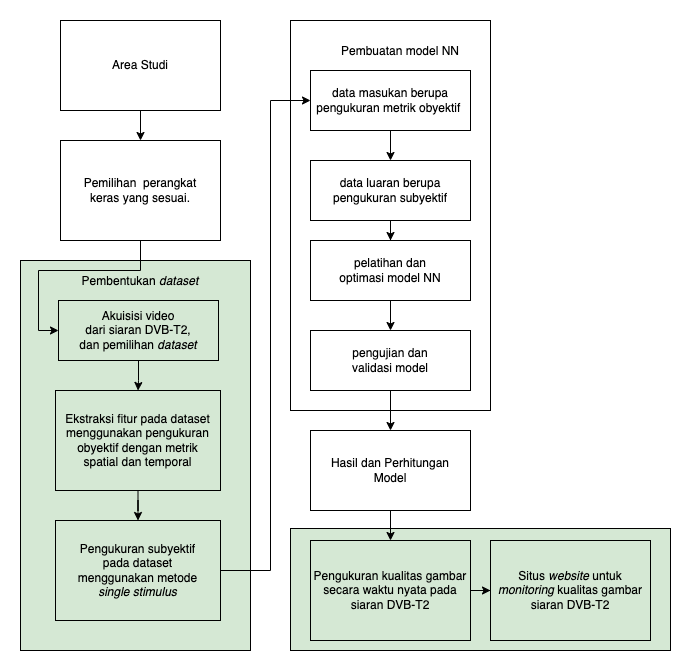
\includegraphics[width=1\columnwidth]{bab3/Gambar/tahapan-penelitian2-1.png}
	\end{center}
	\vspace{-0.2cm}
	%\rule{\columnwidth}{0.1pt}
	\caption{Tahapan penelitian yang dilakukan} \label{tahapan-penelitian}
\end{figure}
%%%%%%%%%%%%%%%%%%%%%%%%%% GAMBAR %%%%%%%%%%%%%%%%%%%%%%%%%%%%%%

Tahap berikutnya adalah dengan membuat model NN dari data pengukuran metrik objektif sebagai parameter masukan, dan data pengukuran subjektif sebagai parameter luaran. Model NN yang dibuat dilakukan dengan melakukan pengujian dari beberapa NN yang ada hingga memperoleh hasil yang sesuai dengan hasil pengukuran subjektif. Proses pembuatan model dilakukan dengan menggunakan Super Komputer DGX A100 milik Universitas Gunadarma. Selanjutnya dilakukan pengukuran akurasi dan korelasi untuk menvalidasi antara hasil dari model dibandingkan dengan pengukuran subyektif. Tahapan terakhir adalah mengimplementasikan hasil pengukuran dan model NN ke dalam perangkat \textit{edge computing}. Perangkat yang digunakan adalah Raspberry Pi 4 dengan tambahan  modul TV \textit{Hat}. Pengukuran kualitas video dapat dilakukan secara waktu nyata pada siaran DVB-T2. Hasil dari pengukuran selanjutnya ditampilan  pada \textit{website} pemantauan.



\section{Area Studi}
\hspace{1,2cm}
Penelitian ini dilakukan di Indonesia lebih tepatnya di Wilayah Kota Depok, Jawa Barat, berbatasan dengan Kota Madya Jakarta Selatan. Proses pengambilan data video dan pengukuran kualitas gambarnya yang diperoleh dari siaran DVB-T2 dilakukan di lokasi Kampus F8, Universitas Gunadarma. Video diambil dengan menggunakan perangkat komputer yang terhubung secara langsung ke siaran DVB-T2 menggunakan\textit{ tv tunner} dan juga antena. 

\subsection{Obyek Penelitian}
\hspace{1,2cm}
Obyek penelitian ini adalah \textit{frame} video definisi tinggi penuh \textit{(Full High Definition, FHD)} yang diperoleh dari siaran televisi DVB-T2. FHD memilki resolusi gambar 1080p atau $1920\times1080$ piksel. Pada penelitian ini durasi pengambilan sampel video sampel pada siaran DVB-T2 hanya 10 detik untuk setiap samplenya, mengikuti standar pengukuran kualitas gambar ITU-R BT.500. Video diambil dari beberapa layanan televisi lokal yang ada di Indonesia, khususnya di wilayah studi. Beberapa layanan tv digital yang didapat seperti Metro TV, Net TV, TVRI World, TVRI, Sport, dan MyTV. Layanan yang dipilih merupakan layanan yang sudah mendukung resolusi video FHD. Pada gambar \Ref{gambar-tvriw} merupakan hasil gambar FHD yang diperoleh dari siaran DVB-T2 menggunakan perangkat komputer. 

%%%%%%%%%%%%%%%%%%%%%%%%%% GAMBAR %%%%%%%%%%%%%%%%%%%%%%%%%%%%%%
\begin{figure}[H]
	\vspace{-0.1cm}
	%\rule{\columnwidth}{0.1pt}
	\begin{center}
		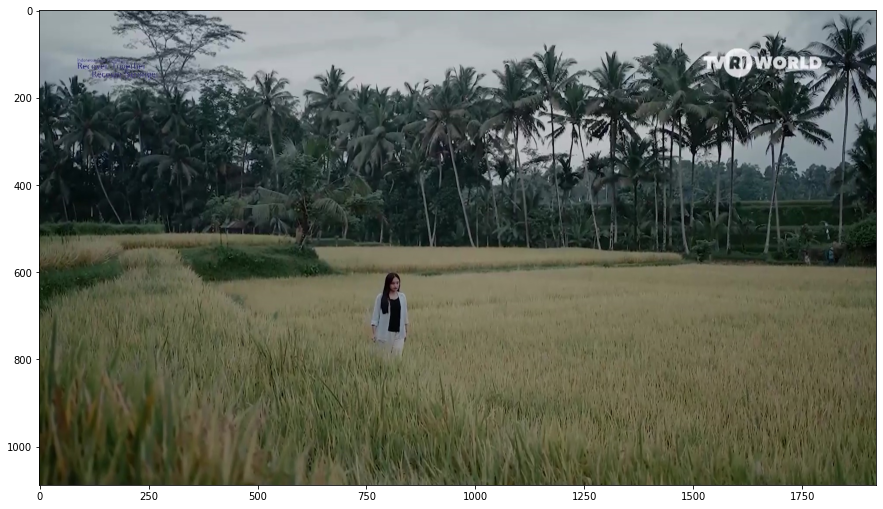
\includegraphics[width=1\columnwidth]{bab3/Gambar/gambar-tvriw.png}
	\end{center}
	\vspace{-0.2cm}
	%\rule{\columnwidth}{0.1pt}
	\caption{Contoh Gambar FHD dari layanan TVRI World} \label{gambar-tvriw}
\end{figure}
%%%%%%%%%%%%%%%%%%%%%%%%%% GAMBAR %%%%%%%%%%%%%%%%%%%%%%%%%%%%%%

Proses pengambilan video membutuhkan beberapa perangkat keras dan perangkat lunak. Perangkat keras yang digunakan adalah perangkat komputer, raspberry pi, \textit{tv tunner}, antena dan monitor. Perangkat lunak yang digunakan adalah \textit{tvheadend}, \textit{visual studio code}, \textit{jupyterlab}, dan bahasa pemprograman \textit{python} beserta librari pendukungnya.


\subsection{Pemilihan Perangkat Keras}
\hspace{1,2cm}
Penelitian ini memiliki beberapa tahapan seperti yang dijelaskan pada gambar \ref{tahapan-penelitian}, sehingga memerlukan perangkat yang mendukung dimulai dari proses pengambilan data, pengukuran obyektif dan subyektif, hingga memperoleh model, dan hasil. Perangkat keras yang digunakan juga tidak hanya satu jenis, dikarena setiap proses pada tahapan penelitian, menggunakan spesifikasi perangkat keras yang berbeda. Proses pengambilan data dan pengujian hasil dilakukan pada perangkat \textit{edge computing} yang terhubung langsung dengan siaran DVB-T2. Sedangkan pada proses pengukuran dan pembuatan model untuk jaringan saraf tiruan (NN) menggunakan perangkat komputer atau cloud computing. Perangkat keras yang digunakan diantaranya:

\begin{itemize}
	\item Perangkat \textit{Edge Computing} untuk pengambilan data dan juga pengukuran secara waktu nyata menggunakan Raspberry Pi 4 model B dengan prosesor Cortex-A72 ARM v8 64-bit up to 1.5 Mhz, VideoCore VI support Openg GL 3.0, dan RAM LPDDR4 8GB.
	\item Perangkat \textit{tv-tunner} untuk \textit{edge computing} yang digunakan adalah raspberry pi TV HAT \textit{(Hardware Attach on Top)} dengan Tuner Sony CXD2880, mendukung DVB-T2 dengan frekuensi pembawa VHF dan UHV, mendukung format video MPEG-2 dan H.264, yang umum digunakan dalam siaran televisi digital.
	\item Perangkat pengukuran video subyektif  yang digunakan adalah Macbook 2019, prosesor intel hexa-core i7 Gen-9, GPU AMD Radeon Pro 555X, RAM DDR4 16GB, layar 15.4 inci resolusi $2880\times1800$.
	\item Perangkat untuk pengukuran dan  membuat model \textit{neural network} menggunakan \textit{Super Computer }NVIDIA DGX A100 dengan virtual machine yang digunakan RAM 20GB dan GPU 40GB
	
\end{itemize}

Pemilihan perangkat komputer yang digunakan sebagai \textit{edge computing} berdasarkan pada kemampuan untuk dapat dapat terhubung langsung dengan modul TV Hat yang bisa menerima siaran televisi digital DVB-T2. Sedangkan perangkat yang digunakan dalam membuat model NN berdasarkan pada kecepatan memproses data dan juga merupakan salah satu fasilitas dari Universitas Gunadarma. Kedua perangkat tersebut menggunakan versi perangkat lunak yang sama untuk memudahkan proses duplikasi program.

%%%%%%%%%%%%%%%%%%%%%%%%%% TABEL %%%%%%%%%%%%%%%%%%%%%%%%%%%%%%
\begin{table}[H]
	\centering
	\caption{Versi bahasa pemprograman python dan librarinya}
	\label{tabel-spek-sw}
	\begin{tabular}{|c|c|c|c|c|c|}
		\hline
		Nama Library & python & opencv & matplotlib & numpy  & tensorflow \\ \hline
		Versi        & 3.8.5  & 4.6.0  & 3.2.2      & 1.21.6 & 2.11.0     \\ \hline
	\end{tabular}
\end{table}
%%%%%%%%%%%%%%%%%%%%%%%%%% TABLE %%%%%%%%%%%%%%%%%%%%%%%%%%%%%%

Fokus dari penelitian terdapat pada sisi penerima siaran televisi digital. Siaran DVB-T2 yang diterima dari antenna menuju \textit{receiver} dan mengalami beberapa tahapan \textit{decoder} untuk memperoleh video dan audio. Frame gambar dari video hasil akhir proses tersebut yang akan diukur dan didapat nilai kualitasnya berdasarkan beberapa parameter.

%%%%%%%%%%%%%%%%%%%%%%%%%% GAMBAR %%%%%%%%%%%%%%%%%%%%%%%%%%%%%%
\begin{figure}[H]
	\vspace{-0.1cm}
	%\rule{\columnwidth}{0.1pt}
	\begin{center}
		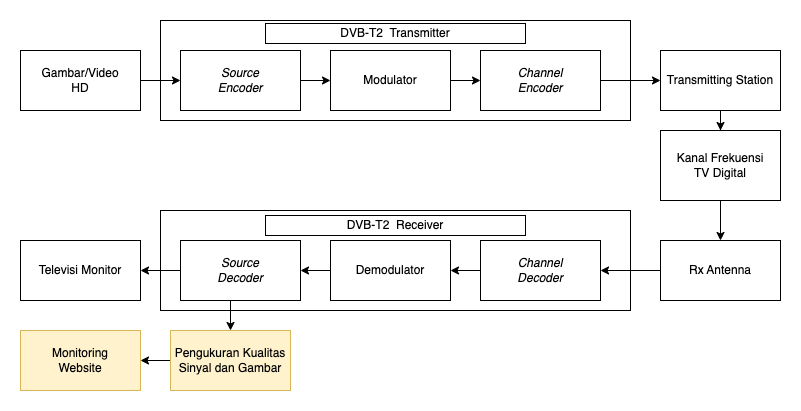
\includegraphics[width=1\columnwidth]{bab3/Gambar/fokus-penelitian.png}
	\end{center}
	\vspace{-0.2cm}
	%\rule{\columnwidth}{0.1pt}
	\caption{Fokus Penelitian} \label{fokus-penelitian}
\end{figure}
%%%%%%%%%%%%%%%%%%%%%%%%%% GAMBAR %%%%%%%%%%%%%%%%%%%%%%%%%%%%%%

Luaran akhir dari penelitian ini adalah mendapat model yang sesuai untuk dapat melakukan pengukuran kualitas gambar pada siaran DVB-T2. Pengukuran juga dilakukan terhadap parameter sinyal dari siaran yang sedang dilakukan pengukuran gambarnya. Hasil dari pengukuran akan secara waktu nyata ditampilkan pada \textit{website} dan tersimpan secara berkala.


\section{Pembentukan \textit{Dataset}}
\hspace{1.2cm}
Dalam mencapai tujuan  dari penelitian maka dibuat sebuah rancangan dari sistem secara keseluruhan. Sistem terdiri dari beberapa perangkat keras dan lunak yang memiliki tugas dan fungsi masing-masing yang saling terhubung. Keterbaruan dari penelitian ini juga adalah sistem secara keseluruhan yang ditunjukkan pada gambar \ref{rancangan-sistem} dan NN untuk dalam proses pengukuran kualitas gambar secara waktu nyata.

%%%%%%%%%%%%%%%%%%%%%%%%%% GAMBAR %%%%%%%%%%%%%%%%%%%%%%%%%%%%%%
\begin{figure}[H]
	\vspace{-0.1cm}
	%\rule{\columnwidth}{0.1pt}
	\begin{center}
		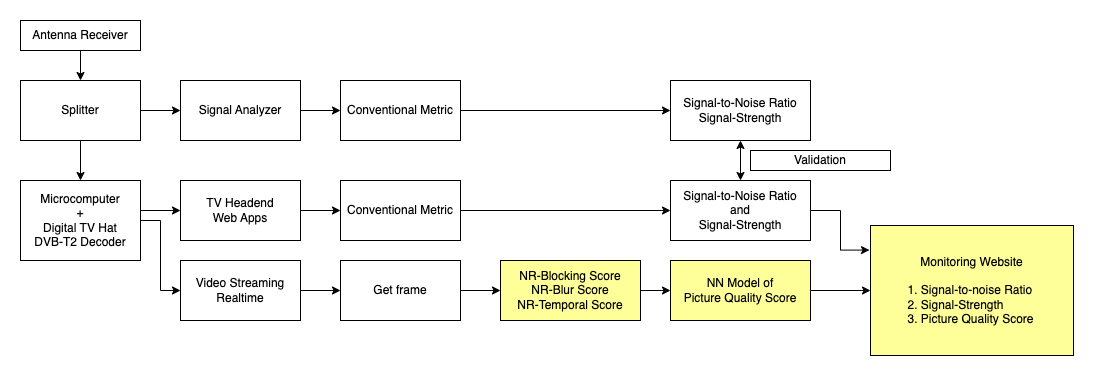
\includegraphics[width=1\columnwidth]{bab3/Gambar/rancangan-sistem.png}
	\end{center}
	\vspace{-0.2cm}
	%\rule{\columnwidth}{0.1pt}
	\caption{Rancangan Sistem Pengukuran Kualitas Gambar Siaran DVB-T2} \label{rancangan-sistem}
\end{figure}
%%%%%%%%%%%%%%%%%%%%%%%%%% GAMBAR %%%%%%%%%%%%%%%%%%%%%%%%%%%%%%

Sistem diawali dari pengambilan sinyal siaran tv digital menggunakan Antenna yang kemudian di split ke dua alat yaitu yang pertama adalah mikro komputer \textit{Raspberry Pi }dengan \textit{tv tunner}, kedua \textit{signal analyzer}. Aplikasi yang digunakan pada raspberry pi adalah \textit{tvheadend} yang berfungsi menampilkan siaran tv digital pada perangkat \textit{rapsberry pi} dan menampilkan status pengukuran sinyalnya. Spectrum analyzer digunakan hanya untuk melakukan validasi pada parameter sinyal siaran tv digital. Selanjutnya dengan menggunakan aplikasi ffmpeg dan pemprograman python setiap video yang sedang ditayangkan dapat diambil frame gambarnya. Frame yang diambil diukur menggunakan obyektif metriks untuk memperoleh parameter input dari kualitas gambar frame tersebut. Hasil pengukuran berupa angka yang nantinya akan dimasukkan ke dalam model NN untuk memperoleh nilai kualitas yang sudah disesuaikan dengan penilaian subyektif manusia. Hasil akhir pengukuran sinyal dan juga kualitas gambar ditampilkan dalam sebuat \textit{website}.

\subsection{Akuisisi \textit{Dataset} Video}
\hspace{1,2cm}
Video yang dijadikan dataset adalah video yang diperoleh dari siaran DVB-T2 secara langsung dengan resolusi HD dan FHD, yaitu resolusi 1280x720 piksel (720p) dan 1920x1080 piksel (1080p). Proses pengambilan video dilakukan dengan menggunakan perangkat keras \textit{Raspberry Pi 4} dengan modul \textit{TV HAT}. Kemudian perangkat tersebut harus terhubung dengan antena televisi agar dapat menerima siaran DVB-T2. Antena yang digunakan pada penelitian ini adalah PX HDA-5000. 

Perangkat lunak yang digunakan dalam proses pengambilan data video adalah \textit{tvheadend}. Aplikasi tersebut dapat menampilkan siaran televisi digital dari tv \textit{tunner} ke perangkat komputer. Aplikasi tvheadend kemudian diatur untuk melakukan perekaman video HD dari siaran televisi digital. Beberapa layanan televisi yang sudah HD diantaranya TVRI HD, TVRI World, Net TV HD dan Metro TV HD. Dalam pengambilan dataset, diambil sejumlah 100 video dari masing-masing layanan tersebut dengan durasi per video adalah 10 detik. 


\subsection{Metrik Obyektif Pengukuran Kualitas Gambar}
\hspace{1,2cm}
Metrik obyektif merupakan suatu ukuran atau parameter yang dapat diukur secara kuantitaf. Pada penelitian digunakan beberapa metrik obyektif untuk melakukan pengukuran pada kualitas video. Metrik obyektif yang digunakan diantarauntuk pengukuran spatial pada gambar seperti  blocking  dan blur, ada juga metrik yang digunakan untuk melakukan pengukuran temporal terhadap frame yang terdapat pada video. Metrik obyektif  juga digunakan untuk melakukan pemilihan dataset dan sebagai parameter masukan yang nantinya digunakan dalam NN.

\subsubsection{Metrik Bloking}
\hspace{1,2cm}
\textit{Blocking} pada gambar adalah efek visual yang terjadi ketika akibat kompresi data yang dilakukan pada gambar atau video dengan mengurangi jumlah bit yang digunakan untuk merepresentasikan piksel di dalamnya. Saat terjadi kerusakan pada bit data tersebut dan gambar didekompresi kembali, maka akan muncul kerusakan seperti  munculnya kotak-kotak besar yang terlihat di dalam gambar, yang disebut sebagai \textit{bloking}. Gambar dengan kondisi \textit{blocking} dapat dilihat pada gambar \ref{gambar-blocking}.

%%%%%%%%%%%%%%%%%%%%%%%%%% GAMBAR %%%%%%%%%%%%%%%%%%%%%%%%%%%%%%
\begin{figure}[H]
	\vspace{-0.1cm}
	%\rule{\columnwidth}{0.1pt}
	\begin{center}
		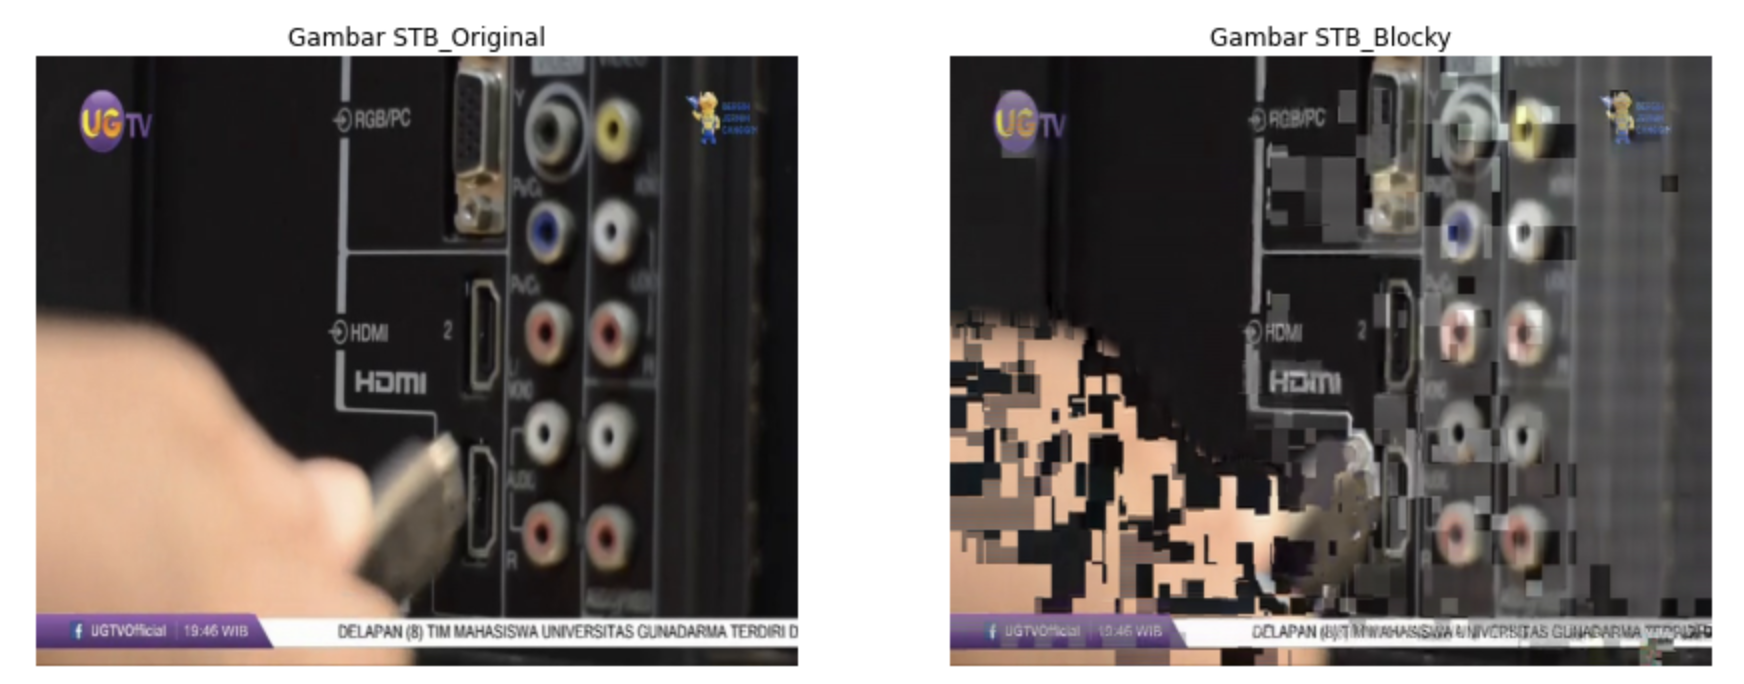
\includegraphics[width=1\columnwidth]{bab3/Gambar/gambar-blocking.png}
	\end{center}
	\vspace{-0.2cm}
	%\rule{\columnwidth}{0.1pt}
	\caption{Perbandingan gambar normal dan \textit{blocking}} \label{gambar-blocking}
\end{figure}
%%%%%%%%%%%%%%%%%%%%%%%%%% GAMBAR %%%%%%%%%%%%%%%%%%%%%%%%%%%%%%


Pada penelitian ini digunakan salah satu algoritma pengukuran tingkat \textit{blocking} pada gambar yang dikemukakan oleh \textit{Zhou Wang}. Teknik pengkodean gambar yang membagi gambar menjadi sub-blok 8x8 piksel. Proses transformasi dan kuantisasi kemudian diterapkan pada masing-masing sub-blok secara individual dan independen. Teknik pengkodean gambar ini umumnya digunakan dalam teknologi kompresi gambar, seperti pada standar kompresi JPEG, dan dapat menyebabkan munculnya artefak blok atau blocking artifact pada gambar. Sehingga pengukuran \textit{bloking} pada gambar dilakukan setiap 8 piksel secara horizontal dan vertikal.

\begin{equation} 
	\label{eq3-1}
	\begin{split}
		&image\_resolution = x(m,n) \\
		&dimana, \ m \in \left[ 1,M \right], \ n\in \left[ 1,N \right]
	\end{split}
\end{equation}

Gambar diubah ke dalam skala keabuan (grayscale) untuk dapat memperoleh satu saluran warna dengan jumlah m baris dan n kolom. Kemudian dilakukan pengukuran secara terpisah antara baris dan kolom. Ide dasar dari algoritma ini adalah untuk mendeteksi sinyal blok dan memperkirakan dayanya dengan menggunakan asumsi bahwa gambar yang berblok adalah gambar yang tidak berblok yang terganggu oleh sinyal blok ideal. Algoritma ini dimulai dengan menghitung selisih antara piksel-piksel sepanjang baris untuk mendapatkan selisih horizontal d\textsubscript{h} dan sepanjang kolom untuk mendapatkan selisih vertikal d\textsubscript{v}. 

\begin{equation} 
	\label{eq3-2}
	d_{h}(m,n)=x(m,n+1)-x(m,n), \ n\in [1, N-1] 
\end{equation}

\begin{equation} 
	\label{eq3-3}
	d_{v}(m,n)=x(m+1,n)-x(m,n), \ n\in [1, M-1]
	\vspace{0.5cm}
\end{equation}

Setelah selisih-selisih ini dihitung, gambar selisih dapat diperoleh. Selanjutnya, keberblokan dihitung dengan mengambil rata-rata selisih di sepanjang batas blok. Untuk gambar berukuran M x N, pengukuran horizontal didefinisikan sebagai persamaan berikut:

\begin{equation} 
	\label{eq3-4}
	B_{h}=\frac{1}{M(\left\lfloor N/8 \right\rfloor-1)}\sum_{i=1}^{M}\sum_{j=1}^{\left\lfloor N/8 \right\rfloor-1}\left| d_h(i,8j) \right|
	\vspace{0.5cm}
\end{equation}

Selanjutkan dilakukan pengukuran tingkat aktifitas sinyal. Aktivitas sinyal gambar mengacu pada ukuran intensitas sinyal atau informasi yang terkandung dalam gambar. Semakin tinggi aktivitas sinyal, semakin banyak detail yang terdapat dalam gambar dan semakin sedikit pengaburan atau keberblokan yang terlihat. Pengukuran aktivitas sinyal dapat membantu dalam mengidentifikasi pengaburan atau keberblokan pada gambar. Pada metode ini dilakukan pengukuran aktifitas sinyal gambar meliputi rata-rata selisih absolut (A) antar sampel gambar di dalam blok dan tingkat  \textit{zero-crossing}  (Z) \citep{Wang2002}.

\begin{equation} 
	\label{eq3-5}
	A_h=\frac{1}{7}\left[\frac{8}{M(N-1)}\sum_{i=1}^{M}\sum_{j=1}^{N-1}\left| d_h(i,j) \right|-B_h\right]
	\vspace{0.5cm}
\end{equation}

Pengukuran aktifitas gambar kedua adalah menghitung rata-rata dari \textit{zero-crossing}. Zero crossing adalah fenomena di mana sinyal atau gelombang melintasi sumbu nol. Hal ini dapat dihitung dengan menghitung jumlah kali di mana sinyal melintasi sumbu nol dalam interval waktu tertentu. Semakin banyak tingkat nol-crossing yang terjadi, semakin tinggi aktivitas sinyal dan semakin banyak detail yang terdapat dalam gambar atau sinyal tersebut. 

\begin{equation} 
	\label{eq3-6}
	z_h(m,n)=\begin{cases}1 & horizontal \ ZC \ pada \ d_h(m,n) \\0 & selain \ itu\end{cases}
	\vspace{0.5cm}
\end{equation}

\begin{equation} 
	\label{eq3-7}
	Z_h=\frac{1}{M(N-2)}\sum_{i=1}^{M}\sum_{j=1}^{N-2} d_h(i,j)
	\vspace{0.5cm}
\end{equation}

Metode yang sama dilakukan pada pengukuran secara vertikal pada B\textsubscript{v}, A\textsubscript{v}, dan Z\textsubscript{v}. Kemudian, rata-rata blockiness, B, rata-rata perbedaan absolut, A, dan rata-rata tingkat \textit{zero crossing,} Z, diperoleh dengan menggunakan pengukuran vertikal dan horizontal yang dijumlahkan dan dibagi dua.

\begin{equation} 
	\label{eq3-8}
	B=\frac{B_h+B_v}{2}, \ A=\frac{A_h+A_v}{2}, \ B=\frac{Z_h+Z_v}{2}
	\vspace{0.5cm}
\end{equation}


Ukuran blockiness akhir, S, kemudian dapat diperoleh menggunakan rumus:
\begin{equation} 
	\label{eq3-9}
	S=\alpha+\beta B^{\gamma_1}A^{\gamma_2}B^{\gamma_3}
	\vspace{0.5cm}
\end{equation}

Dimana  $\alpha, \beta,{\gamma _1}, {\gamma _2}, $ dan $ {\gamma _3}$, mewakili parameter prediksi yang diperoleh melalui fitting kurva data eksperimen subjektif  yang dilakukan oleh Wang. Kemudian berdasarkan algoritma diatas maka dibuatlah program ke dalam bahasa pemprograman python.

\subsubsection{Metrik Blur}
\hspace{1,2cm}
Blur pada gambar adalah kondisi di mana gambar menjadi kurang tajam dan terlihat kabur seperti yang ditunjukkan pada gambar \ref{lena-blur}. Hal ini disebabkan oleh hilangnya komponen frekuensi tinggi pada gambar, yang dapat terjadi karena berbagai faktor seperti pergerakan kamera saat pengambilan gambar atau ketidakfokusan saat pemotretan. Gambar bisa menjadi blur juga karena transmisi, yaitu ketika sinyal gambar dikirimkan melalui jaringan atau media transmisi, seperti kabel atau gelombang radio. Selama transmisi, sinyal gambar dapat terdistorsi atau terganggu oleh kebisingan dan interferensi. Hal ini dapat menyebabkan kehilangan atau penyimpangan data gambar, terutama pada detail halus dan frekuensi tinggi, yang akhirnya menyebabkan gambar tampak blur atau kabur. Kualitas transmisi bergantung pada faktor-faktor seperti kecepatan transfer data, kualitas sinyal, dan jarak antara pemancar dan penerima. 

%%%%%%%%%%%%%%%%%%%%%%%%%% GAMBAR %%%%%%%%%%%%%%%%%%%%%%%%%%%%%%
\begin{figure}[H]
	\vspace{-0.1cm}
	%\rule{\columnwidth}{0.1pt}
	\begin{center}
		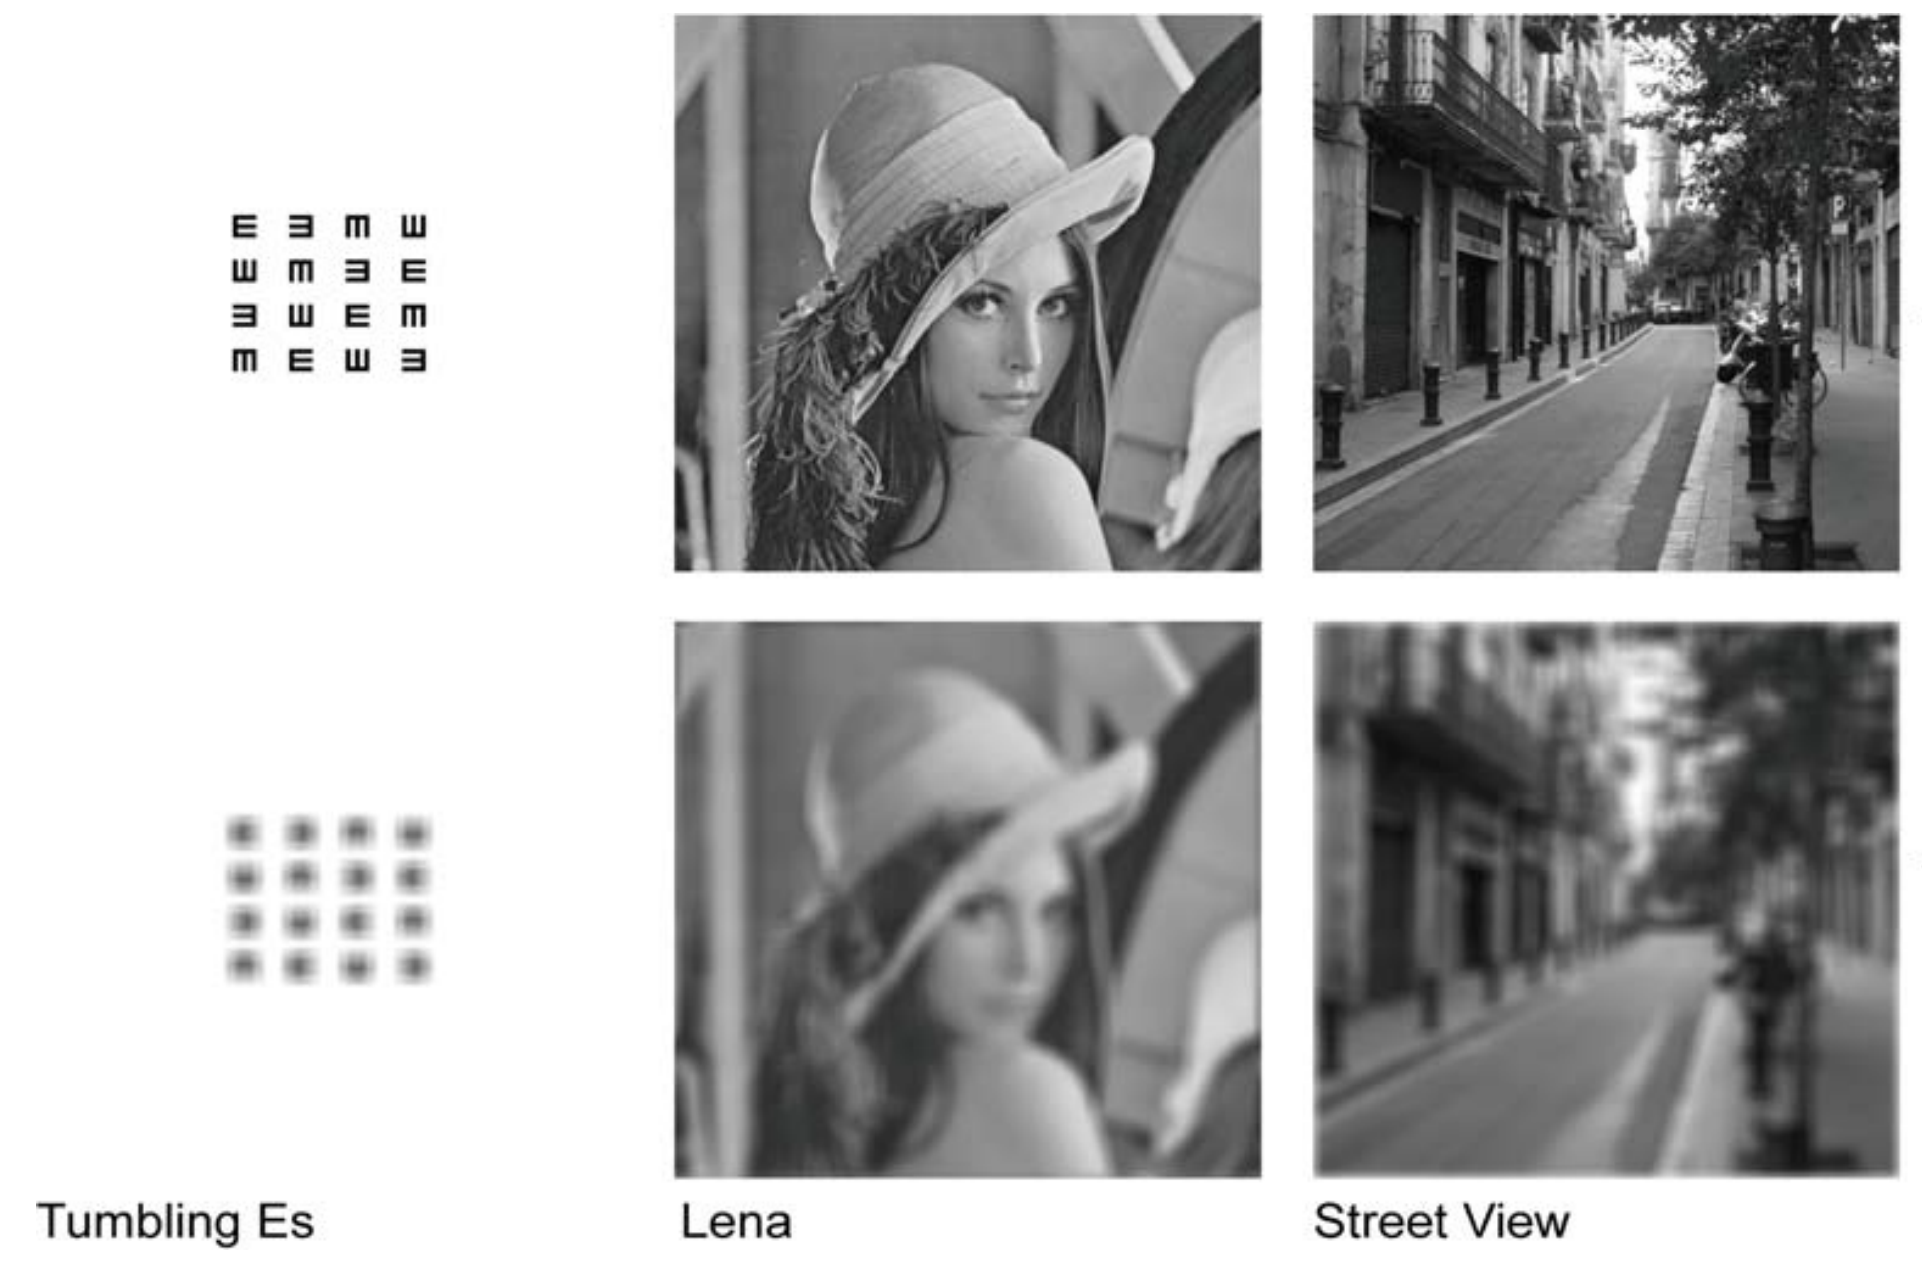
\includegraphics[width=0.8\columnwidth]{bab3/Gambar/lena-blur.png}
	\end{center}
	\vspace{-0.2cm}
	%\rule{\columnwidth}{0.1pt}
	\caption{Perbandingan Gambar Blur dan tidak, dari kiri ke kanan: Tumbling Es, Lena, Street View \citep{Xu_2021}} \label{lena-blur}
\end{figure}
%%%%%%%%%%%%%%%%%%%%%%%%%% GAMBAR %%%%%%%%%%%%%%%%%%%%%%%%%%%%%%

Gejala blur pada gambar dapat diidentifikasi dengan melihat kehalusan tepi atau kekurangan detail halus pada gambar. Terdapat beberapa teknik yang dapat digunakan untuk mengukur tingkat blur pada gambar, salah satunya adalah dengan menggunakan deteksi tepi. Metode ini didasarkan pada observasi bahwa gambar yang kabur memiliki tepian yang kurang tajam atau tidak jelas, karena kehilangan komponen frekuensi tinggi. Oleh karena itu, dengan mendeteksi tepi pada gambar, kita dapat mengukur tingkat kejelasan tepi yang terdapat pada gambar dan menggunakan nilai ini untuk mengindikasikan tingkat blur pada gambar tersebut \citep{Ferzli_2009}. 

Deteksi tepi dapat dilakukan dengan menggunakan algoritma Sobel. Dalam metode ini, gambar diubah menjadi citra grayscale dan dilakukan operasi perataan pada gambar dengan kernel tertentu untuk menghilangkan noise.

\begin{equation} 
	\label{eq3-10}
	G_x = 
	\begin{bmatrix}
		-1 & 0 & +1 \\
		-2 & 0 & +2 \\
		-1 & 0 & +1
	\end{bmatrix} \ \ \ \ \ \ \ \    
	G_y=
	\begin{bmatrix}
		+1 & +2 & +1 \\
		0  & 0  & +2 \\
		-1 & -2 & -1
	\end{bmatrix}\\
	\vspace{0.5cm}
\end{equation}


Selanjutnya, operasi deteksi tepi dilakukan dengan menghitung turunan parsial gambar pada arah vertikal dan horizontal. Hasil dari kedua arah ini kemudian digabungkan dengan menghitung magnitude gradien pada setiap titik pada gambar seperti yang terlihat pada gambar \ref{lenna-edge}. Hasil akhir yang dihasilkan adalah citra biner dengan nilai 0 dan 1, yang menunjukkan lokasi tepi pada gambar.

%%%%%%%%%%%%%%%%%%%%%%%%%% GAMBAR %%%%%%%%%%%%%%%%%%%%%%%%%%%%%%
\begin{figure}[H]
	\vspace{-0.1cm}
	%\rule{\columnwidth}{0.1pt}
	\begin{center}
		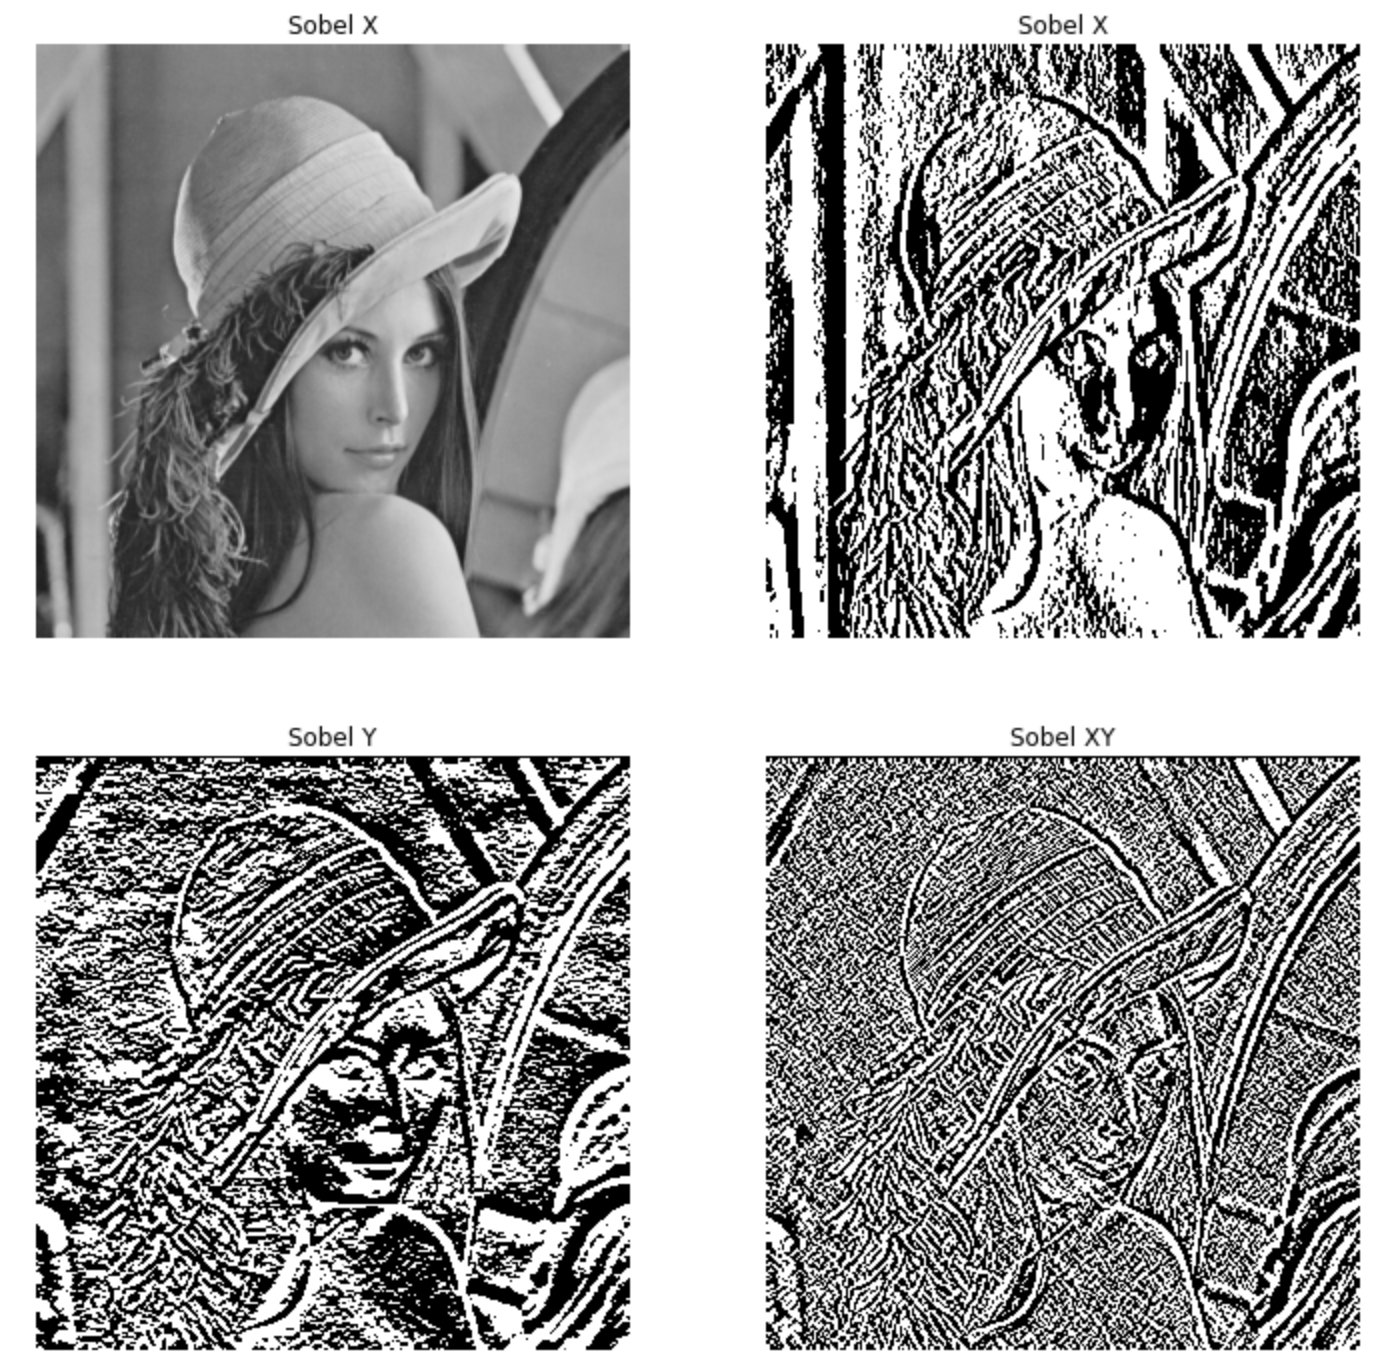
\includegraphics[width=0.8\columnwidth]{bab3/Gambar/lenna-edge.png}
	\end{center}
	\vspace{-0.2cm}
	%\rule{\columnwidth}{0.1pt}
	\caption{Hasil Transformasi ke bentuk deteksi tepi menggunakan sobal pada gambar Lenna} \label{lenna-edge}
\end{figure}
%%%%%%%%%%%%%%%%%%%%%%%%%% GAMBAR %%%%%%%%%%%%%%%%%%%%%%%%%%%%%%

Dalam deteksi tepi, local minimum dan local maximum mengacu pada titik-titik di mana perubahan intensitas mencapai minimum atau maksimum dalam sekelompok piksel pada gambar. Dalam konteks algoritma Marziliano, local minimum dan local maximum digunakan untuk menentukan spread dari tepi vertikal pada gambar yang kabur. Local minimum dan local maximum pada tepi vertikal dihitung pada setiap baris gambar, dan jarak antara kedua titik tersebut memberikan informasi tentang tingkat blur pada gambar \citep{Marziliano}.

Detailnya jika tepi ditemukan, maka lokal ekstremum (maksimum lokal dan minimum lokal) dicari ke arah kiri dan kanan dari piksel tepi. Untuk mencari jarak atau panjang tepi, selisih antara maksimum lokal dan minimum lokal dihitung. Hasilnya diidentifikasi sebagai ukuran blur lokal untuk lokasi tepi saat ini. Akhirnya, ukuran blur global dihitung dengan menghitung rata-rata \textit{blur} lokal di seluruh lokasi tepi. Algoritma dari teknik pengukuran blur ini ditunjukkan pada Gambar \ref{diagram-blur}.

%%%%%%%%%%%%%%%%%%%%%%%%%% GAMBAR %%%%%%%%%%%%%%%%%%%%%%%%%%%%%%
\begin{figure}[H]
	\vspace{-0.1cm}
	%\rule{\columnwidth}{0.1pt}
	\begin{center}
		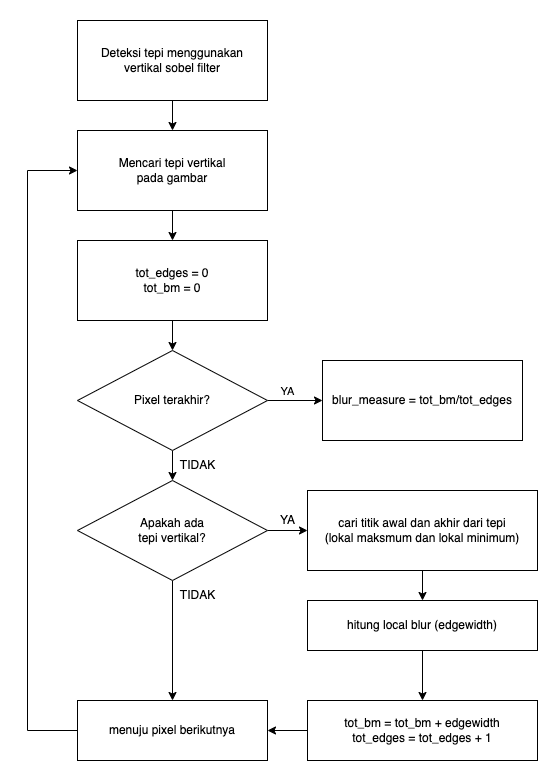
\includegraphics[width=0.6\columnwidth]{bab3/Gambar/algoritma-blur.png}
	\end{center}
	\vspace{-0.2cm}
	%\rule{\columnwidth}{0.1pt}
	\caption{Diagram alur algoritma pengukuran blur pada gambar \citep{Marziliano}} \label{algoritma-blur}
\end{figure}
%%%%%%%%%%%%%%%%%%%%%%%%%% GAMBAR %%%%%%%%%%%%%%%%%%%%%%%%%%%%%%

Metrik pengukuran \textit{blur} tersebut digunakan pada penelitian ini sebagai salah satu parameter masukan untuk pembuatan model NN. Metrik tersebut ditulis kembali menggunakan bahas apemprograman python untuk mempermudah proses pengukuran yang dilakukan pada hardware yang digunakan.

\subsubsection{Metrik Temporal}
\hspace{1,2cm}
Metrik temporal merujuk pada metode pengukuran kualitas video yang fokus pada perubahan dari waktu ke waktu. Metrik ini digunakan untuk mengukur bagaimana perubahan frame dari video yang dihasilkan mempengaruhi kualitas keseluruhan dari video tersebut. Beberapa faktor yang dapat mempengaruhi metrik temporal meliputi jumlah frame yang hilang atau rusak, kualitas gambar pada setiap frame, dan kehalusan perpindahan antar frame. Metrik temporal dapat digunakan untuk mengukur kualitas video pada berbagai jenis aplikasi, termasuk video streaming dan komunikasi video.

Pendekatan umum untuk mendeteksi frame yang beku adalah dengan menghitung mean-squared error (MSE) antara frame saat ini dan frame sebelumnya, dan mempertimbangkan frame saat ini sebagai frame yang beku jika MSE=0. Pertama, video input dikonversi ke ruang warna YUV. Frame yang potensial beku kemudian diidentifikasi berdasarkan MSE antara frame saat ini dan frame sebelumnya:

\begin{equation}
	\begin{aligned}
		YM_{1}(i)=\frac{1}{W*H}\sum_{x=0}^{W-1}\sum_{y=0}^{H-1}(Y(x,y,i)-Y(x,y,i-1))^{2}
	\end{aligned}
\end{equation}

\begin{equation}
	\begin{aligned}
		UM_{1}(i)=\frac{1}{W*H}\sum_{x=0}^{W-1}\sum_{y=0}^{H-1}(U(x,y,i)-U(x,y,i-1))^{2}
	\end{aligned}
\end{equation}

\begin{equation}
	\begin{aligned}
		VM_{1}(i)=\frac{1}{W*H}\sum_{x=0}^{W-1}\sum_{y=0}^{H-1}(V(x,y,i)-V(x,y,i-1))^{2}
	\end{aligned}
\end{equation}

Dimana:
\newline
$Y$ 	\hspace{0.4cm}: saluran warna \textit{luminance}\newline
$U$ 	\hspace{0.4cm}: sarulan warna \textit{chrominance} hijau ke merah \newline
$V$ 	\hspace{0.4cm}: sarulan warna \textit{chrominance} biru ke kuning \newline
$M$ 	\hspace{0.3cm}: veriabel pengukuran antar frame \newline
$W$ 	\hspace{0.3cm}: lebar resolusi gambar \newline
$H$ 	\hspace{0.4cm}: panjang resolusi gambar \newline
$x$ 	\hspace{0.5cm}: piksel baris pada gambar \newline
$y$ 	\hspace{0.4cm}: piksel kolom pada gambar\newline
$i$ 	\hspace{0.5cm}: jumlah frame dalam video (i = 2,...,n) \newline

Konten dengan gerakan sangat rendah dapat menghasilkan MSE yang sangat kecil antara \textit{frame} yang berurutan meskipun \textit{frame} ini tidak beku (\textit{freeze}). Untuk membatasi jumlah positif palsu, mekanisme berikut diterapkan: jika sebuah \textit{frame} berpotensi dibekukan maka \textit{frame} tersebut juga diperiksa terhadap \textit{frame} pertama dari peristiwa pembekuan (kecuali jika \textit{frame} saat ini juga merupakan \textit{frame} pertama dari peristiwa pembekuan). $YM_2(i)$, $UM_2(i)$ dan $VM_2(i)$ menunjuk MSE (masing-masing dalam bidang warna Y, U dan V) antara \textit{frame} saat ini dan \textit{frame} pertama dari peristiwa pembekuan\citep{Quan_Huynh_Thu_2009}.

\begin{equation}
	\begin{aligned}
		YM_{2}(i)=\frac{1}{W*H}\sum_{x=0}^{W-1}\sum_{y=0}^{H-1}(Y(x,y,i)-Y(x,y,i-k))^{2}
	\end{aligned}
\end{equation}

\begin{equation}
	\begin{aligned}
		UM_{2}(i)=\frac{1}{W*H}\sum_{x=0}^{W-1}\sum_{y=0}^{H-1}(U(x,y,i)-U(x,y,i-k))^{2}
	\end{aligned}
\end{equation}

\begin{equation}
	\begin{aligned}
		VM_{2}(i)=\frac{1}{W*H}\sum_{x=0}^{W-1}\sum_{y=0}^{H-1}(V(x,y,i)-V(x,y,i-k))^{2}
	\end{aligned}
\end{equation}

di mana $(i-k)$ adalah indeks temporal dari \textit{frame} pertama dari peristiwa pembekuan di mana \textit{frame} $i$ berada. Sebuah \textit{frame} $i$ akan ditandai sebagai beku jika MSE antara \textit{frame} sekarang dan \textit{frame} sebelumnya tetapi juga antara \textit{frame} ini dan \textit{frame} pertama dari \textit{event freeze} berada dibawah \textit{threshold} T yang sangat kecil dimana \textit{threshold} T ditetapkan ke 1  \citep{Quan_Huynh_Thu_2009}.

\begin{equation}
	\begin{aligned}
		FreezeFlag=\left\{\begin{matrix}
			1 & if(YM,UM,VM)_{1,2}(1)<T  \\
			0 & lainnya \\
		\end{matrix}\right.
	\end{aligned}
\end{equation}

Selanjutnya, nilai durasi freze dijumlahkan untuk memperolah nilai seberapa besar freeze yang terjadi dalam interveal waktu tertentu. Metrik untuk mendeteksi kebekuan pada video ini juga dituliskan dalam bahasa pemprograman phthon sebagai parameter masukan.

\subsection{Pengukuran Subyektif Kualitas Gambar}
\hspace{1,2cm}
Subyektif assessment adalah metode pengukuran yang melibatkan partisipasi manusia untuk memberikan penilaian kualitatif terhadap suatu produk atau layanan berdasarkan pengalaman mereka secara langsung. Dalam konteks pengolahan citra atau video, subyektif assessment dapat digunakan untuk mengukur kualitas visual dari hasil pengolahan tersebut berdasarkan persepsi pengguna. Pada penelitian ini digunakan standar pengukuran subyektif berdasarkan rekomendasi ITU-R BT.500-14 yang diterbitkan Oktober 2019. Standar tersebut menyediakan pedoman dan prosedur untuk penilaian subyektif kualitas gambar televisi \citep{IRB2019}. 

\subsubsection{Single Stimulus Standar ITU-R 500-14}
\hspace{1,2cm}
Single stimulus methods (SS) dipilih sebagai salah satu metode subjective assessment pada ITU-R BT.500-14 karena lebih mudah dilakukan dan lebih efisien dalam hal waktu. Metode ini hanya memerlukan satu gambar  atau video per \textit{sample} sebagai stimulus, sehingga tidak memerlukan waktu yang lama dalam proses evaluasi. Selain itu, metode ini juga tidak memerlukan gambar referensi atau acuan, sehingga lebih fleksibel dan dapat digunakan dalam berbagai kondisi yang berbeda. Meskipun demikian, single stimulus methods juga memiliki kekurangan yaitu rentan terhadap bias pengamat, sehingga perlu dilakukan pengujian ulang dan dilakukan dengan panelis yang berbeda untuk menghasilkan hasil yang lebih akurat dan konsisten.

Metode Single Stimulus dapat digunakan untuk mengevaluasi kualitas video dan gambar. Namun, karena video adalah sekuens gambar yang saling terkait, maka pada pengujian video, stimulus yang diberikan pada setiap pengujian harus sesuai dengan konteks dari adegan yang dipresentasikan. Hal ini bisa dilakukan dengan memilih frame yang mewakili adegan atau dengan memilih klip video pendek yang mewakili adegan tersebut \citep{Seshadrinathan_2010}.

Terdapat beberapa persyaratan pengukuran Single Stimulus (SS) pada ITU-R BT.500-14 yang terdiri dari beberapa hal, antara lain:

\begin{enumerate}
	\item Pemilihan materi uji yang representatif dan bervariasi, serta disajikan dalam kondisi yang sama untuk semua panelis.
	\item Jumlah panelis minimal 15 orang, yang diwajibkan untuk memenuhi syarat tertentu, seperti usia, pengalaman dalam menonton televisi, kesehatan mata, dan tidak memiliki kecacatan warna.
	\item Prosedur pelatihan yang ketat untuk panelis dalam memberikan penilaian yang konsisten dan obyektif.
	\item Penggunaan skala pengukuran yang sesuai, yaitu skala likert yang terdiri dari 5 hingga 7 pilihan untuk menilai kualitas gambar.
	\item Pelaksanaan pengujian dan pengolahan data dengan standar yang ketat dan terdokumentasi dengan baik.
\end{enumerate}

Selain dari faktor pemilihan panelis dan materi uji, standar ITU-R BT.500-14 memberikan panduan yang mencakup beberapa faktor, seperti cahaya lingkungan, warna dinding, dan pencahayaan ruangan yang diperlukan untuk  memastikan konsistensi dan validitas penilaian subjektif. Selain itu, panduan ini juga menyarankan penggunaan layar televisi yang sesuai dengan kondisi pengujian dan memberikan instruksi tentang posisi penonton dan jarak pandang yang optimal. Tujuannya adalah untuk meminimalkan faktor-faktor yang dapat memengaruhi hasil penilaian subjektif dan memastikan bahwa penilaian dilakukan dalam kondisi yang optimal untuk memberikan hasil yang akurat dan dapat diandalkan. Panduan ini sangat penting untuk memastikan bahwa hasil penilaian subjektif kualitas gambar televisi dapat dipertanggungjawabkan dan diandalkan untuk digunakan dalam pengembangan produk dan teknologi baru dalam industri televisi.

Pada pengujiannya dipilih standar \textit{home environment} dengan alasan konteks penggunaan yang lebih realistis dibandingkan dengan di lab, biaya pengujian yang lebih renda, dan waktu yang lebih fleksibel disesuaian dengan panelis. Namun tetap terdapat  beberapa syarat untuk pengujian SS dengan \textit{home environment} yang ditunjukkan pada tabel??.

%%%%%%%%%%%%%%%%%%%%%%%%%% TABLE %%%%%%%%%%%%%%%%%%%%%%%%%%%%%%
\begin{table}[H]
	\centering
	\caption{Standar pengujian SS dengan \textit{home-environment}}
	\label{tabel-ss}
	\begin{tabular}{|l|c|}
		\hline
		\begin{tabular}[c]{@{}l@{}}Penerangan sekitar pada layar \\ (cahaya insiden dari lingkungan \\ yang jatuh pada layar harus diukur \\ secara tegak lurus ke layar\end{tabular} & 200 lux                                                                     \\ \hline
		\begin{tabular}[c]{@{}l@{}}Pencahayaan puncak dari layar \\ (peak luminance)\end{tabular}                                                                                     & 70-500 lux                                                                  \\ \hline
		\begin{tabular}[c]{@{}l@{}}Rasio pencahaayan antara \\ kondisi layar tidak aktif dan \\ kondisi layar puncak\end{tabular}                                                     & $\le 0.02$                                                                  \\ \hline
		Resolusi gambar/video                                                                                                                                                         & $1920\times1080$                                                            \\ \hline
		Aspect rasio                                                                                                                                                                  & 16:9                                                                        \\ \hline
		Sudut lihat optimal dari layar                                                                                                                                                & $31^\circ$                                                                  \\ \hline
		Jarak lihat optimal dari layar                                                                                                                                                & \begin{tabular}[c]{@{}c@{}}3.2 H\\ (H = lebar gambar di layar)\end{tabular} \\ \hline
		Durasi keseluruhan pengujian                                                                                                                                                  & $\le 30$  menit                                                             \\ \hline
	\end{tabular}
	
\end{table}
%%%%%%%%%%%%%%%%%%%%%%%%%% TABLE %%%%%%%%%%%%%%%%%%%%%%%%%%%%%%

Pada umumnya durasi klip yang digunakan berkisar antara 5 hingga 10 detik. Durasi ini dianggap cukup untuk menampilkan adegan yang mewakili isi dari keseluruhan konten. Selain itu, durasi klip yang terlalu lama dapat membuat panelis cepat lelah dan mempengaruhi konsistensi hasil penilaian. Oleh karena itu, durasi klip perlu dipertimbangkan secara cermat untuk memastikan keakuratan dan konsistensi dari hasil penilaian \citep{IRB2019}.

\subsubsection{Tahap 1 - Pemilihan materi dan luaran}

\hspace{1,2cm}
Sebelum memulai pengujian subyektif dipilih terlebih dahulu materi/video yang akan dinilai. Video dipilih dari dataset yang sudah diambil dari siaran DVB-T2. Jumlah materi/video klip yang diujikan sebanyak 105 video FHD dengan durasi per video 10 detik. Perangkat yang digunakan dalam proses pengujian adalah Macbook Pro 2019 dengan ukuran layar 16 inci. Penilaian pada video uji menggunakan skala kualitas gambar ITU-R yang ditunjukkan pada tabel \ref{tabel-skala-quality}.   

%%%%%%%%%%%%%%%%%%%%%%%%%% TABLE %%%%%%%%%%%%%%%%%%%%%%%%%%%%%%
\begin{table}[H]
	\centering
	\caption{Skala ITU-R Quality dan Impairment}
	\label{tabel-skala-quality}
	\begin{tabular}{|ll|}
		\hline
		\multicolumn{2}{|c|}{Skala lima kelas}                              \\ \hline
		\multicolumn{1}{|c|}{Quality}     & \multicolumn{1}{c|}{Impairment} \\ \hline
		\multicolumn{1}{|l|}{5 Excellent} & 5 Imperceptible                 \\ \hline
		\multicolumn{1}{|l|}{4 Good}      & 4 Perceptible, but not annoying \\ \hline
		\multicolumn{1}{|l|}{3 Fair}      & 3 Slightly annoying             \\ \hline
		\multicolumn{1}{|l|}{2 Poor}      & 2 Annoying                      \\ \hline
		\multicolumn{1}{|l|}{1 Bad}       & 1 Very annoying                 \\ \hline
	\end{tabular}
\end{table}
%%%%%%%%%%%%%%%%%%%%%%%%%% TABLE %%%%%%%%%%%%%%%%%%%%%%%%%%%%%%

Luaran dari subyektif assessment pada gambar siaran televisi berupa skala pengukuran. Terdapat dua jenis skala pengukuran, yaitu skala kualitas dan skala \textit{impairment}. Skala kualitas digunakan untuk mengukur sejauh mana penonton merasakan kualitas gambar atau video yang ditampilkan. Skala ini biasanya berbentuk angka atau kata-kata yang merepresentasikan level kualitas. Responden diminta untuk memilih nilai yang paling sesuai dengan pengalaman menonton mereka. Sedangkan skala impairment digunakan untuk mengukur sejauh mana gangguan pada gambar atau video memengaruhi kualitas tampilan secara keseluruhan. Responden diminta untuk memilih nilai yang paling sesuai dengan tingkat gangguan pada gambar atau video. Dalam beberapa kasus, skala kualitas dan skala \textit{impairment} digunakan bersamaan untuk memberikan gambaran yang lebih lengkap tentang kualitas gambar atau video yang ditampilkan \citep{Mittal_2012}.

\subsubsection{Tahap 2 - Sesi tes}
\hspace{1,2cm}
Terdapat dua bagian pada tes seperti yang ditunjukkan pada gambar \ref{structure-tes}, yang pertama adalah urutan latihan atau \textit{training sequence}, dan selanjutnya sesi tes (test session). \textit{Training sequence} atau urutan latihan berupa serangkaian langkah atau instruksi yang diberikan kepada panelis dalam rangka melatih mereka untuk melakukan penilaian subyektif dengan konsisten dan akurat. \textit{Training sequence} biasanya mencakup langkah-langkah seperti familiarisasi dengan peralatan pengujian, instruksi tentang melaksanakan tugas penilaian, dan latihan tentang mengenali dan mengevaluasi aspek-aspek kualitas gambar yang berbeda. Langkah ini penting untuk memastikan bahwa panelis memahami dan menggunakan skala penilaian dengan konsisten dan bahwa hasil penilaian subyektif akurat dan dapat diandalkan. 

%%%%%%%%%%%%%%%%%%%%%%%%%% GAMBAR %%%%%%%%%%%%%%%%%%%%%%%%%%%%%%
\begin{figure}[H]
	\vspace{-0.1cm}
	%\rule{\columnwidth}{0.1pt}
	\begin{center}
		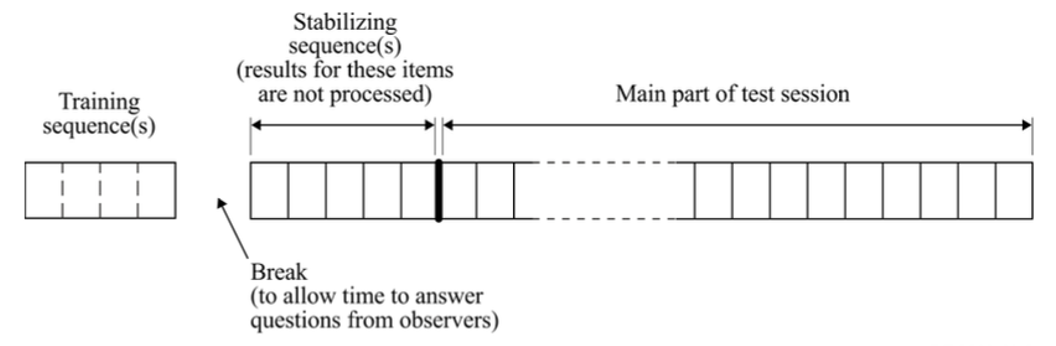
\includegraphics[width=1\columnwidth]{bab3/Gambar/structure-tes.png}
	\end{center}
	\vspace{-0.2cm}
	%\rule{\columnwidth}{0.1pt}
	\caption{Struktur presentasi dari subyektif tes} \label{structure-tes}
\end{figure}
%%%%%%%%%%%%%%%%%%%%%%%%%% GAMBAR %%%%%%%%%%%%%%%%%%%%%%%%%%%%%%

Pada awal sesi pertama, sekitar lima "presentasi \textit{dummy}" harus diperkenalkan untuk menstabilkan pendapat para pengamat. Data yang dihasilkan dari presentasi ini tidak boleh dipertimbangkan dalam hasil pengujian. Selanjutnya secara langsung tanpa sepengetahuan pengamat dilakukan bagian utama dari sesi tes. Setiap presentasi diawali dan diakhiri dengan \textit{midgrey} yang diantara berupa materi uji. \textit{Midgrey} merupakan citra dengan nilai keabuan antara putih dan hitam dengan nilai RGB (128,128,128) atau HEX \#808080. Mid-grey biasanya digunakan sebagai referensi dalam pengujian subyektif untuk mengevaluasi kualitas kontras, ketajaman, dan keseimbangan warna.

Durasi yang umumnya digunakan adalah sekitar 10 detik untuk materi uji dan 1 hingga 2 detik untuk \textit{midgrey}. Durasi ini dapat disesuaikan tergantung pada kebutuhan pengujian dan karakteristik materi uji yang digunakan. Waktu antara \textit{midgrey} dan materi uji pada penelitian adalah 1, 10, dan 3 detik seperti yang ditunjukkan pada gambar \ref{midgrey-time}.

%%%%%%%%%%%%%%%%%%%%%%%%%% GAMBAR %%%%%%%%%%%%%%%%%%%%%%%%%%%%%%
\begin{figure}[H]
	\vspace{-0.1cm}
	%\rule{\columnwidth}{0.1pt}
	\begin{center}
		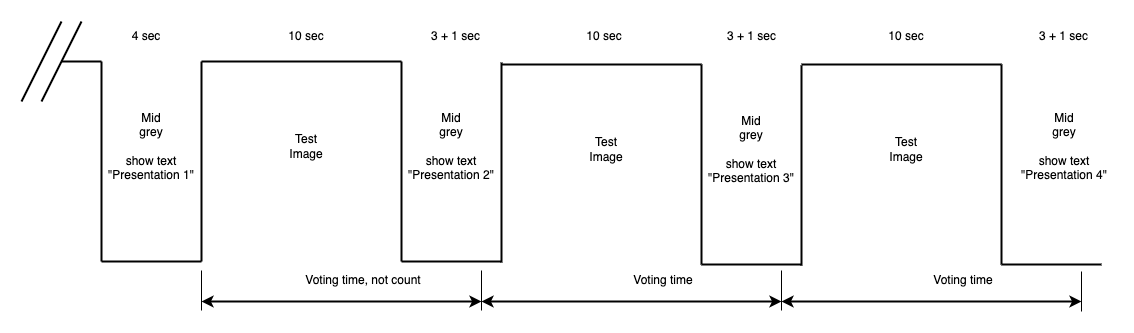
\includegraphics[width=1\columnwidth]{bab3/Gambar/midgrey-time.png}
	\end{center}
	\vspace{-0.2cm}
	%\rule{\columnwidth}{0.1pt}
	\caption{Interval antara \textit{midgrey} dan materi uji} \label{midgrey-time}
\end{figure}
%%%%%%%%%%%%%%%%%%%%%%%%%% GAMBAR %%%%%%%%%%%%%%%%%%%%%%%%%%%%%%

Berdasarkan interval tersebut maka dapat dihitung jumlah waktu yang dibutuhkan untuk menyelesaikan rangkaian pengukuran subyektif. Jumlah materi yang digunakan sesi tes termasuk \textit{dummy} sebanyak 100 + 5 video klip. Waktu yang dibutuhkan dalam 1 video adalah 14 detik termasuk dengan \textit{midgrey}. Sehingga waktu yang dibutuhkan sebanyak $105\times14 = 1470$ detik atau sekitar 24.5 menit. Jika ditambah dengan \textit{training sequence} yang membutuhkan waktu 3-5 menit, maka total waktu yang dibutuhkan untuk melakukan rangkaian secara keseluruhan masih $\le 30$ menit.


\subsubsection{Tahap 3 - Pengukuran hasil tes}
\hspace{1,2cm}
Pengukuran hasil pengukuran subyektif  \textit{single stimulus}melibatkan sejumlah panelis yang menilai kualitas gambar dari materi uji pada layar monitor. Skor subyektif diberikan dan dianalisis untuk menentukan rata-rata skor, standar deviasi, dan interval kepercayaan. Materi uji terdiri dari beberapa klip video yang dipilih secara acak dari berbagai jenis siaran televisi, yang ditampilkan dalam urutan acak. Panelis diberikan klip latihan sebelumnya untuk membiasakan diri dengan tampilan antarmuka dan jenis gambar yang akan dinilai. Skor diberikan pada skala kualitas ITU-R dengan 1 menunjukkan kualitas gambar yang sangat buruk dan 5 menunjukkan kualitas gambar yang sangat baik. Hasil pengukuran dapat digunakan untuk mengevaluasi kualitas gambar pada siaran televisi dengan menghitung skor rata-rata, standar deviasi, dan interval kepercayaan \citep{IRP2022}.

Pengukuran hasil yang pertama adalah mengukur rata-rata dari setiap materi yang dipresentasikan ke panelis, dengan persamaan berikut:

\begin{equation}
	\begin{aligned}
		\bar{u}_{ijkr}=\frac{1}{N}\sum_{i=1}^{N}u_{ijkr}
	\end{aligned}
\end{equation}

\hspace{-1,2cm}dimana:
\vspace{-0.5cm}
\begin{tabbing}
	$\bar{u}_{ijkr}$ \hspace{2em} \= : nilai dari panelis i untuk kondisi tes j, urutan ke k, pengulangan r \\
	$N$ \> : jumlah panelis \\
\end{tabbing}
\vspace{-0.5cm}

Demikian pula, skor rata-rata keseluruhan, $u_j$ dan $u_k$, dapat dihitung untuk setiap kondisi uji dan setiap urutan/gambar uji. Selanjutnya saat menyajikan hasil pengujian, semua skor rata-rata harus memiliki interval kepercayaan yang terkait yang berasal dari standar deviasi dan ukuran masing-masing sampel. Berdasarkan ITU-R BT.500-14 dianjurkan untuk menggunakan interval kepercayaan 95\% yang dinyatakan sebagai berikut:

\begin{equation}
	\begin{aligned}
		\left[ \bar{u}_{jkr}-\delta_{jkr}, \bar{u}_{jkr}+\delta_{jkr} \right]
	\end{aligned}
\end{equation}

\hspace{-1,2cm}dimana:
\vspace{0.5cm}
\begin{equation}
	\begin{aligned}
		\delta_{jkr}=1.96 \frac{S_{jkr}}{N}
	\end{aligned}
\end{equation}
\vspace{0.25cm}

\hspace{-1,2cm}Standar deviasi untuk setiap presentasi $S_{jkr}$ dapat dinyatakan dalam persamaan:
\begin{equation}
	\begin{aligned}
		{S_{jkr}}=\sqrt{\sum_{i=1}^{N}\frac{(\bar{u}_{jkr}-\bar{u}_{ijkr})^{2}}{(N-1)}}
	\end{aligned}
\end{equation}
\vspace{0.25cm}

Dengan probabilitas 95\%, nilai mutlak dari selisih antara skor rata-rata eksperimental dan skor rata-rata sebenarnya (untuk jumlah pengamat yang sangat tinggi) lebih kecil dari interval kepercayaan 95\%, asalkan distribusi skor individual memenuhi persyaratan tertentu. Demikian pula, deviasi standar $S_j$ dapat dihitung untuk setiap kondisi uji. Namun, perlu dicatat bahwa deviasi standar ini, dalam kasus penggunaan jumlah urutan/gambar uji yang sedikit, akan lebih dipengaruhi oleh perbedaan antara urutan/gambar uji yang digunakan daripada variasi antara penilai yang berpartisipasi dalam penilaian.


\subsubsection{Desain Aplikasi Subyektif \textit{Assessment}}
\hspace{1,2cm}
Subyektif \textit{assessment} yang dilakukan untuk pengukuran kualitas gambar menggunakan perangkat lunak berbasis \textit{local website}. Perangkat lunak dirancang untuk memudahkan proses pengambilan data dan juga memudahkan panelis dalam melakukan penilaian. Pada awal tampilan terdapat pilihan antara \textit{training sequence} dan sesi tes. Pada tampilan utama saat tes terdapat jendela pemutaran materi video dan juga tab penilaian seperti yang ditunjukkan pada gambar \ref{single_stimulus} rancangan aplikasi subyektif \textit{assessment}. Rangkaian materi video dan \textit{mid-grey} akan ditampilkan secara berkala sesuai dengan skema yang sudah direncanakan.

%%%%%%%%%%%%%%%%%%%%%%%%%% GAMBAR %%%%%%%%%%%%%%%%%%%%%%%%%%%%%%
\begin{figure}[H]
	\vspace{-0.1cm}
	%\rule{\columnwidth}{0.1pt}
	\begin{center}
		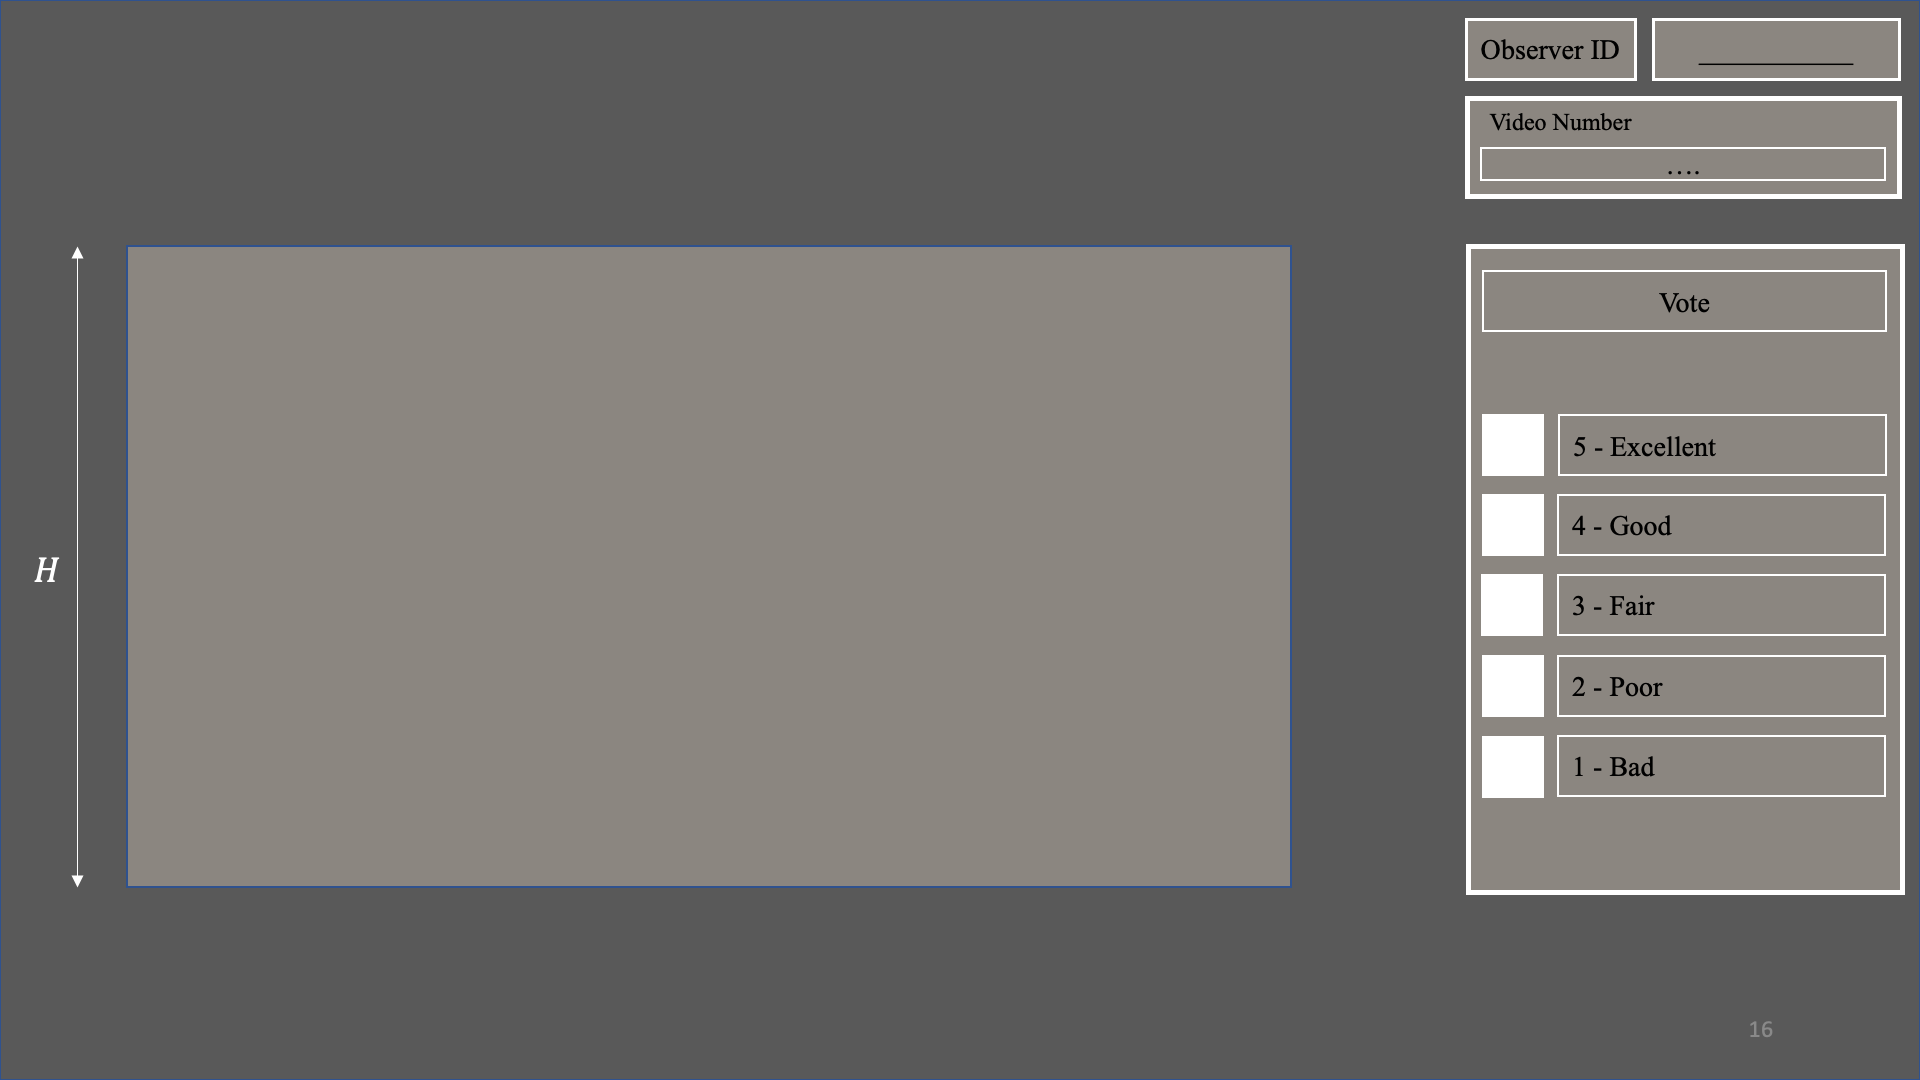
\includegraphics[width=1\columnwidth]{bab3/Gambar/single_stimulus.png}
	\end{center}
	\vspace{-0.2cm}
	%\rule{\columnwidth}{0.1pt}
	\caption{Rancangan tampilan aplikasi web subyektif \textit{assessment}} \label{single_stimulus}
\end{figure}
%%%%%%%%%%%%%%%%%%%%%%%%%% GAMBAR %%%%%%%%%%%%%%%%%%%%%%%%%%%%%%

Aplikasi ditujukan untuk mempermudah proses pengujian pada subyektif \textit{assessment}. Beberapa fitur yang dibutuhkan seperti melakukan input materi video yang akan diujikan, melakukan pengambilan datadan perekaman jawaban dari panelis, dan menarik keseluruhan data uji hasil evaluasi serta dapat di export ke dalam format .csv. Setiap panelis juga memilki ID masing-masing sehingga data bisa dikelompokkan berdasarkan panelis atau berdasarkan materi yang diujikan.




\section{Pembuatan Model NN}
\hspace{1,2cm}
Jaringan saraf tiruan \textit{(Neural network, NN)} digunakan dalam subyektif \textit{assessment} untuk memprediksi kualitas gambar atau video berdasarkan fitur-fitur tertentu. Proses pembuatan model NN dimulai dengan pemilihan fitur-fitur yang relevan dengan kualitas gambar atau video yang ingin diprediksi. Fitur-fitur tersebut dapat berupa metrik kualitas gambar seperti metrik \textit{blocking}, metrik \textit{blur}, dan metrik \textit{temporal}. Setelah pemilihan fitur, langkah selanjutnya adalah pemilihan arsitektur dan parameter untuk model NN. Pada penelitian ini dipilih \textit{Recurrent Neural Network (RNN)} untuk memodelkan hubungan antara penilaian kualitas gambar/video oleh manusia dengan fitur-fitur gambar/video yang dijadikan input pada model seperti yang ditunjukkan pada gambar \ref{tahap-nn}. Diharapkan penilaian kualitas gambar/video yang dihasilkan oleh model dengan RNN lebih akurat karena model dapat mengambil informasi sebelumnya pada urutan input yang diberikan.

%%%%%%%%%%%%%%%%%%%%%%%%%% GAMBAR %%%%%%%%%%%%%%%%%%%%%%%%%%%%%%
\begin{figure}[H]
	\vspace{-0.1cm}
	%\rule{\columnwidth}{0.1pt}
	\begin{center}
		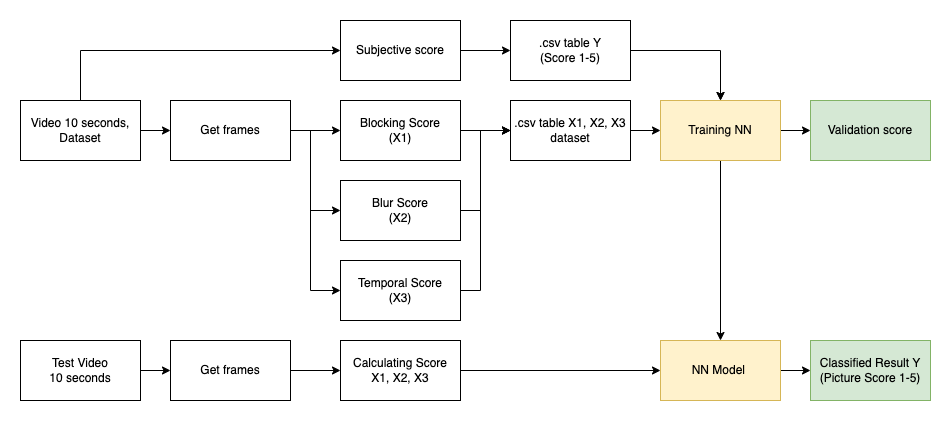
\includegraphics[width=1\columnwidth]{bab3/Gambar/tahap-nn.png}
	\end{center}
	\vspace{-0.2cm}
	%\rule{\columnwidth}{0.1pt}
	\caption{Diagram parameter I/O untuk membangun model NN} \label{tahap-nn}
\end{figure}
%%%%%%%%%%%%%%%%%%%%%%%%%% GAMBAR %%%%%%%%%%%%%%%%%%%%%%%%%%%%%%
 
Setelah arsitektur dan parameter ditentukan, langkah selanjutnya adalah pelatihan model NN menggunakan data latih yang telah dilabeli dengan nilai kualitas yang sesuai. Data latih harus mencakup variasi yang cukup dari kualitas gambar atau video yang ingin diprediksi. Setelah model dilatih, kinerjanya dievaluasi menggunakan data uji yang belum pernah dilihat oleh model \citep{Otroshi_Shahreza_2019}. Berikut proses dan tahapan untuk membangun arsitektur NN yang akan dilakukan pada penelitan ini meliputi:

\begin{enumerate}
	\item Menentukan masukan (input) dan keluaran (output) dari model: Langkah pertama adalah menentukan jenis data masukan yang akan digunakan dan keluaran yang diharapkan dari model. 
	
	\item Memilih arsitektur NN: Berdasarkan jenis masukan dan keluaran yang telah ditentukan, kemudian dipilih arsitektur NN yang tepat.
	
	\item Menentukan jumlah lapisan dan neuron: Setelah memilih arsitektur NN yang tepat, selanjutnya ditentukan jumlah lapisan dan neuron pada setiap lapisan. Jumlah lapisan dan neuron ini dapat disesuaikan dengan kompleksitas data dan sumber daya komputasi yang tersedia.
	
	\item Menentukan fungsi aktivasi: Fungsi aktivasi digunakan untuk mengaktifkan neuron pada setiap lapisan. Beberapa fungsi aktivasi yang umum digunakan adalah sigmoid, relu, dan tanh.
	
	\item Mengatur hyperparameter: Hyperparameter adalah parameter yang diatur sebelum memulai pelatihan model. Beberapa hyperparameter yang perlu diatur adalah learning rate, batch size, dan jumlah epoch.
	
	\item Pelatihan model: Setelah menentukan arsitektur NN dan hyperparameter, selanjutnya model dilatih dengan menggunakan data latih. Proses pelatihan ini dilakukan dengan mengoptimalkan fungsi loss yang dihasilkan.
	
	\item Evaluasi model: Setelah selesai dilatih, model dievaluasi dengan menggunakan data uji untuk mengevaluasi performa dan akurasi model. Apabila hasil evaluasi masih belum memuaskan, dapat dilakukan iterasi kembali pada tahap pelatihan model atau penyesuaian parameter lainnya.
	
	\item Prediksi atau inferensi: Setelah model dievaluasi dan dianggap cukup baik, model dapat digunakan untuk memprediksi nilai output dari data yang baru atau melakukan inferensi.
	
	\item Penggunaan dan pemeliharaan model: Setelah berhasil dibuat, model dapat digunakan untuk memproses data yang baru. Namun, model juga perlu dipelihara secara berkala agar tetap optimal dalam memproses data.
\end{enumerate}

%%%%%%%%%%%%%%%%%%%%%%%%%% GAMBAR %%%%%%%%%%%%%%%%%%%%%%%%%%%%%%
\begin{figure}[H]
	\vspace{-0.1cm}
	%\rule{\columnwidth}{0.1pt}
	\begin{center}
		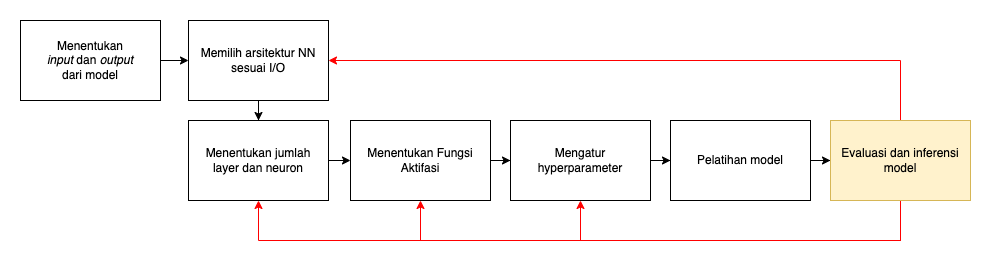
\includegraphics[width=1\columnwidth]{bab3/Gambar/langkah-model.png}
	\end{center}
	\vspace{-0.2cm}
	%\rule{\columnwidth}{0.1pt}
	\caption{Tahapan pembuatan arsitektur dan model NN}
	\label{langkah-model}
\end{figure}
%%%%%%%%%%%%%%%%%%%%%%%%%% GAMBAR %%%%%%%%%%%%%%%%%%%%%%%%%%%%%%

Seluruh tahapan dilakukan dalam penelitian ini untuk memperoleh model RNN yang tepat seperti pada gambar \ref{langkah-model}. Seperti memilih jenis RNN yang sesuai dengan jenis data dan tugas yang akan dilakukan. Beberapa jenis RNN yang umum digunakan adalah LSTM, GRU, dan SimpleRNN. Kemudian penentuan hyperparameter seperti jumlah neuron, learning rate, jumlah epochs, dan batch size sangat penting untuk membangun model yang optimal. Evaluasi model secara sistematis setelah model dibangun, model harus dievaluasi secara sistematis menggunakan metrik yang tepat seperti akurasi, presisi, dan recall. Hal ini dapat membantu memastikan bahwa model dapat digunakan dengan efektif untuk tugas yang diberikan.


\section{Hasil dan Perhitungan Model}
\hspace{1.2cm}
Setelah model NN terbentuk, yang perlu dilakukan adalah melakukan pengukuran model tersebut. Akurasi, presisi, \textit{recall}, \textit{F1-score}, \textit{confusion matrix}, dan \textit{loss function} merupakan parameter yang perlu diukur pada model NN. Akurasi dihitung dengan membandingkan nilai prediksi dengan nilai sebenarnya pada data uji. Presisi dihitung dengan membagi jumlah prediksi positif benar dengan jumlah keseluruhan prediksi positif. Recall dihitung dengan membagi jumlah prediksi positif benar dengan jumlah keseluruhan data positif pada data uji. \textit{F1-score} merupakan ukuran gabungan antara presisi dan \textit{recall} dan dihitung dengan menghitung rata-rata harmonis antara presisi dan recall.

\subsection{\textit{Confusion} matriks}
\hspace{1.2cm}
\textit{Confusion matrix} digunakan untuk mengevaluasi performa model NN dengan memperlihatkan jumlah prediksi benar dan salah yang dibuat oleh model. Confusion matrix digunakan untuk menghitung akurasi, presisi, dan \textit{recall}. \textit{Loss function} merupakan fungsi yang digunakan untuk mengukur seberapa besar kesalahan prediksi model pada setiap iterasi selama proses pelatihan. Loss function digunakan untuk mengoptimalkan bobot pada model NN. Semua parameter ini penting untuk mengukur dan mengevaluasi performa model NN dalam memprediksi hasil pengukuran subyektif pada sistem monitoring kualitas siaran DVB-T2.

Pada penelitian ini terdapat 5 klasifikasi pada hasil NN, yaitu nilai kualitas 1 sampai 5 berdasarkan ITU-R. Sehingga digunakan \textit{multiple class confusion matrix} (MCCM) untuk mengevaluasi performa dari model NN. Sama seperti confusion matrix sederhana terdapat juga parameter TP, TN, FP, dan FN  yang merupakan empat nilai dalam confusion matrix yang digunakan untuk mengevaluasi performa model pada tugas klasifikasi. 

\begin{itemize}
	\item TP (true positive) adalah jumlah kasus positif yang terdeteksi dengan benar oleh model.
	\item TN (true negative) adalah jumlah kasus negatif yang terdeteksi dengan benar oleh model.
	\item FP (false positive) adalah jumlah kasus negatif yang salah terdeteksi sebagai positif oleh model.
	\item FN (false negative) adalah jumlah kasus negatif yang salah terdeteksi sebagai negatif oleh model.
\end{itemize}

%%%%%%%%%%%%%%%%%%%%%%%%%% GAMBAR %%%%%%%%%%%%%%%%%%%%%%%%%%%%%%
\begin{figure}[H]
	\vspace{-0.1cm}
	%\rule{\columnwidth}{0.1pt}
	\begin{center}
		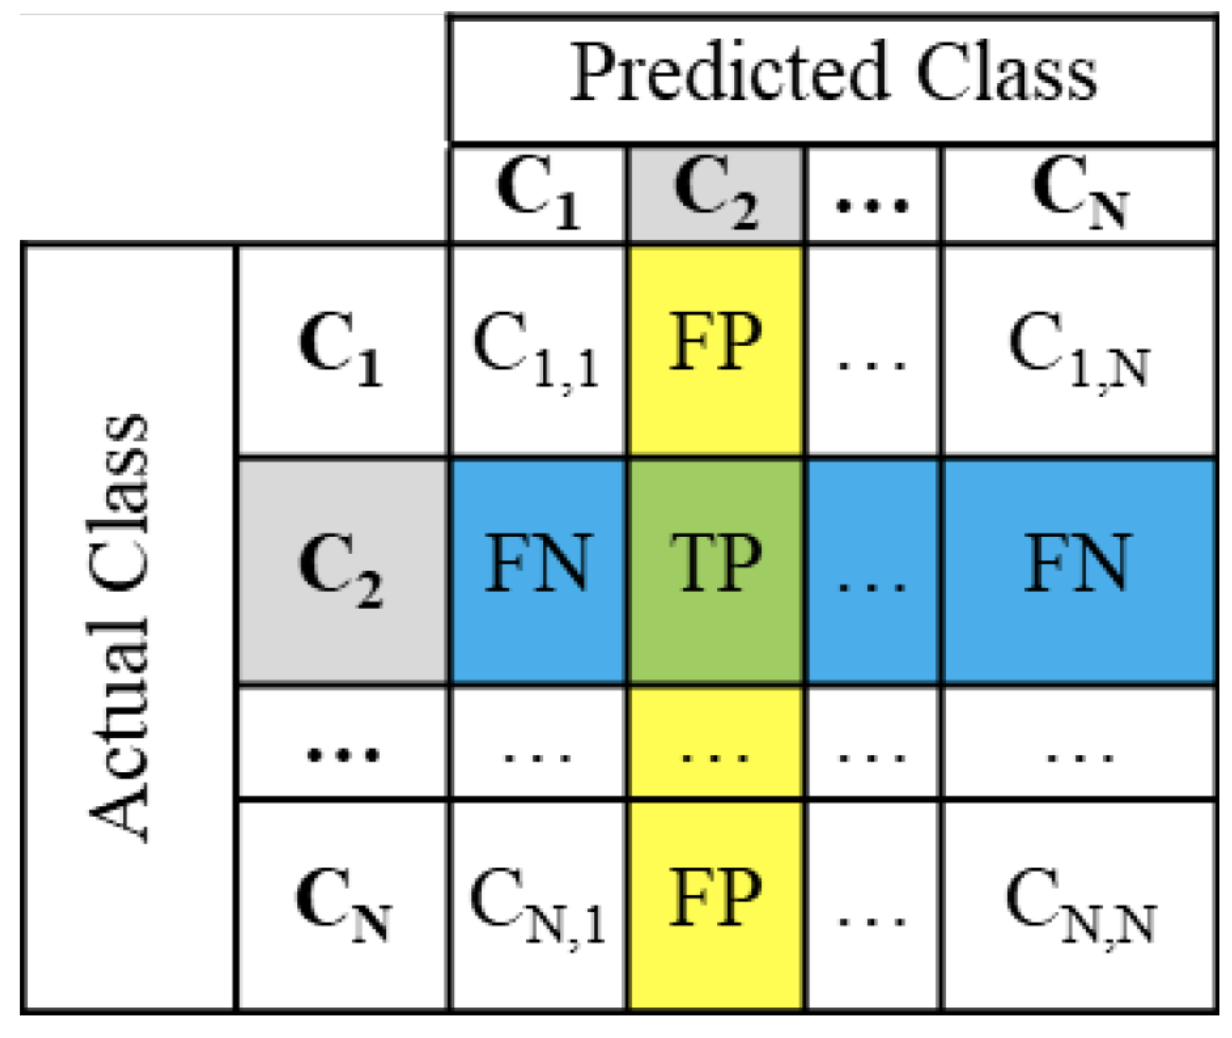
\includegraphics[width=0.5\columnwidth]{bab3/Gambar/mc-cm.png}
	\end{center}
	\vspace{-0.2cm}
	%\rule{\columnwidth}{0.1pt}
	\caption{\textit{Multiple Class Confusion Matrix} \citep{Markoulidakis_2021}}
	\label{mc-cm}
\end{figure}
%%%%%%%%%%%%%%%%%%%%%%%%%% GAMBAR %%%%%%%%%%%%%%%%%%%%%%%%%%%%%%


Dalam konteks MCCM, TP, TN, FP, dan FN dihitung berdasarkan kelas target dan prediksi yang berbeda pada data uji yang memiliki lebih dari dua kelas. Diagonal matriks MCCM menunjukkan jumlah prediksi benar untuk setiap kelas, sementara sel di luar diagonal menunjukkan jumlah prediksi salah untuk setiap kelas seperti yang ditunjukkan pada gambar \ref{mc-cm}. Oleh karena itu, TP, TN, FP, dan FN pada MCCM terdapat pada setiap sel matriks dan digunakan untuk menghitung akurasi, presisi, dan recall pada setiap kelas.
Akurasi digunakan untuk mengukur seberapa sering model NN dapat memprediksi dengan benar kelas target pada seluruh data uji \citep{Powers2020}. Menghitung akurasi pada MCCM dapat dilakukan dengan menjumlahkan seluruh TP dibagi dengan seluruh data pada matriks, atau dapat dituliskan dalam rumus:

\begin{equation}
	\begin{aligned}
		Akurasi=\frac{\sum_{i=1}^{k}TP_i}{\sum_{i=1}^{k}(TP_i+FP_i)}
	\end{aligned}
\end{equation}

\hspace{-1,2cm}dimana:
\vspace{-0.5cm}
\begin{tabbing}
	$TP_{i}$ \hspace{2em} \= : jumlah prediksi model yang benar dari kelas $i$\\
	$FP_{i}$ \> : jumlah prediksi model yang salah pada kelas $i$. \\
	$k$ \> : jumlah kelas pada model $i$. \\
\end{tabbing}
\vspace{-0.5cm}

Presisi digunakan mengukur seberapa sering model NN dapat memprediksi dengan benar kelas positif dari semua prediksi positif yang dibuat. Presisi dapat dianggap sebagai tingkat ketepatan dari prediksi positif model NN. Rumus untuk menghitung presisi adalah sebagai berikut:

\begin{equation}
	\begin{aligned}
		Presisi_i =\frac{TP_i}{(TP_i+FP_i)}
	\end{aligned}
\end{equation}

Kemudian untuk menghitung \textit{recall} atau True Positive Rate (TPR) atau sensitivitas, adalah metrik kinerja yang digunakan untuk mengukur seberapa baik model klasifikasi mengidentifikasi hasil positif yang benar dari keseluruhan hasil positif yang sebenarnya. Recall dihitung dengan menggunakan rumus berikut:

\begin{equation}
	\begin{aligned}
		Recall_i =\frac{TP_i}{(TP_i+FN_i)}
	\end{aligned}
\end{equation}

Parameter berikutnya adalah F1-score, merupakan metrik kinerja yang digunakan untuk mengukur kinerja model klasifikasi, terutama dalam situasi di mana distribusi kelas tidak seimbang. F1-score merupakan rata-rata harmonik dari presisi dan recall, yang memperhitungkan keduanya dalam satu metrik. Rumus F1-score:

\begin{equation}
	\begin{aligned}
		F1-score_i =2 \frac{Presisi_i*Recall_i}{(Presisi_i +Recall_i)}
	\end{aligned}
\end{equation}

Dalam konteks klasifikasi multi-kelas, presisi, \textit{recall}, dan \textit{f1-score} dihitung untuk setiap kelas secara terpisah dan kemudian digabungkan menggunakan metode seperti rata-rata sederhana \textit{(macro-average)}, rata-rata mikro \textit{(micro-average)}, atau rata-rata tertimbang \textit{(weighted average)}, tergantung pada konteks masalah dan jumlah sampel per kelas. 

Rumus rata-rata sederhana \textit{(macro-average)}:

\begin{equation}
	\begin{aligned}
		Average_{macro} = \frac {\sum_{i=1}^{k}Metrik_i}{k}
	\end{aligned}
\end{equation}

Rumus rata-rata mikro \textit{micro-average}:

\begin{equation}
	\begin{aligned}
		Average_{micro} =\frac{\sum_{i=1}^{k}TP_i}{(\sum_{i=1}^{k}TP_i+\sum_{i=1}^{k}FP_i)}
	\end{aligned}
\end{equation}


Rumus rata-rata tertimbang \textit{weighted-average}:

\begin{equation}
	\begin{aligned}
		Average_{weighted} =\frac{\sum_{i=1}^{k}(Metrik_i\times Bobot_i)}{(\sum_{i=1}^{k}Bobot_i)}
	\end{aligned}
\end{equation}

Memilih rata-rata yang tepat untuk klasifikasi multi-kelas bergantung pada konteks masalah dan tujuan evaluasi. Macro-average memberikan bobot yang sama pada setiap kelas, cocok untuk menekankan kinerja seimbang di semua kelas, terutama ketika ada ketidakseimbangan kelas yang signifikan. Micro-average memberikan bobot yang sama pada setiap sampel, lebih cocok jika Anda lebih peduli tentang kinerja model secara keseluruhan daripada kinerja kelas individu. Weighted average memberikan bobot yang proporsional terhadap jumlah sampel per kelas, lebih memperhatikan kinerja kelas yang lebih besar dalam evaluasi.

\subsection{Pengukuran Korelasi}
\hspace{1.2cm}
Korelasi antara pengukuran subyektif dan obyektif dapat digunakan untuk mengevaluasi sejauh mana metode pengukuran obyektif dapat memprediksi pengukuran subyektif yang dilakukan oleh manusia. Dengan mengetahui korelasi antara hasil pengukuran subyektif dan objektif, kita dapat mengevaluasi seberapa baik pengukuran objektif dapat merepresentasikan penilaian kualitas gambar atau video oleh manusia. Untuk mengukur korelasi antara pengukuran subyektif dan obyektif, seringkali digunakan koefisien korelasi Pearson. Koefisien korelasi Pearson mengukur hubungan linier antara dua variabel, dalam hal ini pengukuran subyektif dan obyektif. Koefisien ini memiliki nilai antara -1 hingga 1, di mana 1 menunjukkan hubungan positif sempurna, -1 menunjukkan hubungan negatif sempurna, dan 0 menunjukkan tidak ada hubungan linier antara kedua variabel. 

Selain koefisien korelasi Pearson, terdapat juga metode pengukuran korelasi lainnya yang dapat digunakan, seperti koefisien korelasi Spearman dan koefisien korelasi Kendall. Korelasi Spearman juga merupakan salah satu jenis korelasi yang digunakan untuk mengukur hubungan antara dua variabel. Korelasi Spearman menghitung koefisien korelasi rho ($\rho$) antara peringkat dua variabel yang tidak berdistribusi normal atau tidak memiliki asumsi normal \citep{Pinson2004}. Korelasi Spearman dapat digunakan untuk mengukur korelasi antara nilai subyektif dan obyektif dalam penilaian kualitas video atau gambar. 

Berikut rumus yang digunakan untuk menghitung nilai koefisien korelasi Pearson:

\begin{equation}
	\begin{aligned}
		r _xy= \frac{\sum_{i=1}^n (x_i - \bar{x})(y_i - \bar{y})}{\sqrt{\sum_{i=1}^n (x_i-\bar{x})^2 \sum_{i=1}^n (y_i - \bar{y})^2}}
	\end{aligned}
\end{equation}

\hspace{-1,2cm}dimana:
\vspace{-0.5cm}
\begin{tabbing}
	$r_xy$ \hspace{2em} \= : koefisien korelasi Pearson $i$\\
	$x_{i}$ \> : nilai dari variabel x dalam sample $i$. \\
	$\bar{x}$ \> : rata-rata variabel x. \\
	$y_{i}$ \> : nilai dari variabel y dalam sample $i$. \\
	$\bar{x}$ \> : rata-rata variabel y. \\
	$n$ \> : jumlah sample. \\
\end{tabbing}
\vspace{-0.5cm}

Sedangkan untuk menghitung nilai koefisien korelasi Spearman digunakan rumus sebagai berikut:

\begin{equation}
	\begin{aligned}
		\rho = 1 - \frac{6 \sum_{i=1}^n d_i^2}{n(n^2 - 1)}
	\end{aligned}
\end{equation}

\hspace{-1,2cm}dimana:
\vspace{-0.5cm}
\begin{tabbing}
	$\rho$ \hspace{2em} \= : koefisien korelasi peringkat Spearman $i$\\
	$d_{i}$ \> : perbedaan antara peringkat variabel X dan Y pada observasi ke-$i$. \\
	$n$ \> : jumlah sample. \\
\end{tabbing}
\vspace{-0.5cm}

Korelasi Pearson dan Spearman merupakan metode yang berbeda untuk mengukur hubungan antara dua variabel. Korelasi Pearson mengukur hubungan linier antara variabel dengan menggunakan nilai aktual, dan mengasumsikan distribusi normal serta hubungan linier. Sementara itu, korelasi Spearman mengukur hubungan monoton dengan menggunakan peringkat variabel, dan tidak mengharuskan distribusi normal atau hubungan linier, sehingga lebih cocok untuk data ordinal atau data yang tidak berdistribusi normal \citep{Akoglu2018}.

\section{Sistem Pengukuran Waktu Nyata}
\hspace{1.2cm}
Sistem pengukuran waktu nyata pada kualitas gambar siaran DVB-T2 dilakukan setelah didapat model yang dapat melakukan pengukuran dengan tingkat akurasi yang cukup tinggi dibandingkan dengan penilaian subyektif manusia. Prosedur yang dilakukan dalam melakukan pengukuran waktu nyata seperti yang digambarkan pada gambar \ref{realtime-measurement}. Hardware yang digunakan adalah raspberry pi 4 model B dengan menggunakan TV HAT dan juga antena. Raspberry pi sudah terisntall raspbian OS 64-bit, dan sudah diinstall aplikasi \textit{tvheadend}, \textit{ffmpeg}, dan juga \textit{python} dengan \textit{library}-nya.

%%%%%%%%%%%%%%%%%%%%%%%%%% GAMBAR %%%%%%%%%%%%%%%%%%%%%%%%%%%%%%
\begin{figure}[H]
	\vspace{-0.1cm}
	%\rule{\columnwidth}{0.1pt}
	\begin{center}
		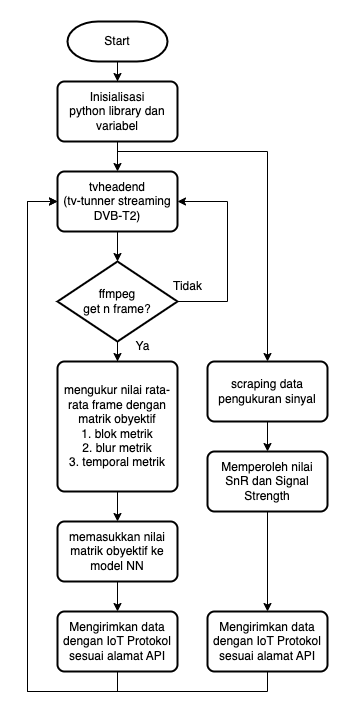
\includegraphics[width=0.6\columnwidth]{bab3/Gambar/realtime-measurement.png}
	\end{center}
	\vspace{-0.2cm}
	%\rule{\columnwidth}{0.1pt}
	\caption{Diagram alur program python pada pengukuran kualitas gambar siaran DVB-T2 waktu nyata}
	\label{realtime-measurement}
\end{figure}
%%%%%%%%%%%%%%%%%%%%%%%%%% GAMBAR %%%%%%%%%%%%%%%%%%%%%%%%%%%%%%

Pertama gambar ditangkap dari  web aplikasi \textit{tvheadend} yang diperoleh langsung pada siaran DVB-T2. Gambar ditangkap menggunakan aplikasi \textit{ffmpeg} yang sudah diprogram menggunakan python untuk melakukan pengambilan data gambar dengan interval tertentu secara berkala. Gambar yang diambil merupakan urutan frame video sebanyak 5 frame dengan interval 0.5 detik. Frame gambar tersebut kemudian diukur satu persatu menggunakan metrik obyektif blur, blok, dan temporal. Hasil pengukuran obyektif  dirata-ratakan kemudian digunakan sebagai parameter masukan pada model NN. Nilai yang diperoleh dari model NN selanjutnya akan dikirim ke IoT dashboard menggunakan protokol IoT seperti \textit{thingspeak} milik \textit{Matlab}. 


\subsection{Tahapan pembuatan \textit{website} pemantauan}
\hspace{1,2cm}
Web aplikasi monitoring kualitas penyiaran DVBT-2 merupakan sebuah aplikasi web yang dapat digunakan untuk memonitor kualitas penyiaran televisi secara waktu nyata \textit{real-time}. Aplikasi ini dapat menampilkan informasi tentang kualitas siaran seperti kualitas video dan kualitas sinyal. Aplikasi ini dilengkapi dengan fitur-fitur seperti pemantauan kualitas siaran secara real-time, pemantauan kualitas siaran secara historis, analisis data kualitas siaran, serta notifikasi jika terjadi gangguan atau perbaikan dalam kualitas siaran. Web aplikasi ini dapat berguna bagi stasiun televisi atau radio untuk memastikan bahwa kualitas siaran yang mereka kirimkan kepada pemirsa adalah yang terbaik, serta memastikan bahwa siaran tidak mengalami gangguan atau masalah teknis. Tahapan dari pembuatan web ditunjuukan pada gambar 

%%%%%%%%%%%%%%%%%%%%%%%%%% GAMBAR %%%%%%%%%%%%%%%%%%%%%%%%%%%%%%
\begin{figure}[H]
	\vspace{-0.1cm}
	%\rule{\columnwidth}{0.1pt}
	\begin{center}
		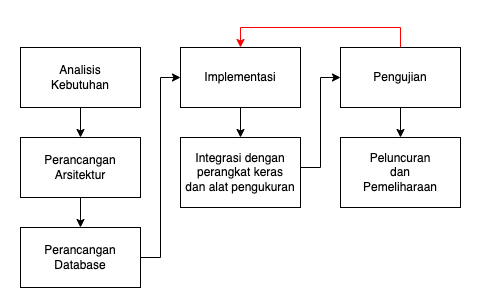
\includegraphics[width=0.8\columnwidth]{bab3/Gambar/pembuatan-web.png}
	\end{center}
	\vspace{-0.2cm}
	%\rule{\columnwidth}{0.1pt}
	\caption{Tahapan pembuatan \textit{website monitoring real-time} kualitas gambar DVB-T2}
	\label{pembuatan-web}
\end{figure}
%%%%%%%%%%%%%%%%%%%%%%%%%% GAMBAR %%%%%%%%%%%%%%%%%%%%%%%%%%%%%%

Perancangan sistem web aplikasi monitoring televisi digital melibatkan beberapa tahapan yang harus dilakukan secara terstruktur. Tahapan pertama adalah melakukan analisis kebutuhan untuk menentukan fitur dan fungsi yang diperlukan dalam aplikasi. Analisis kebutuhan dilakukan dengan mengumpulkan informasi dari stakeholder dan melakukan studi literatur. Selanjutnya, dilakukan perancangan arsitektur sistem, yang mencakup infrastruktur server, database, dan interaksi antarmuka pengguna dengan sistem. Arsitektur ini harus dirancang dengan mempertimbangkan aspek keamanan, skalabilitas, dan kinerja sistem.

Setelah perancangan arsitektur, dilakukan perancangan database untuk menyimpan data yang dibutuhkan oleh aplikasi, seperti data pengguna, data channel televisi, dan data kualitas sinyal. Tahapan selanjutnya adalah implementasi, yang mencakup pembuatan kode program, integrasi komponen sistem, pengujian, dan debugging. Penting juga untuk melakukan integrasi dengan perangkat perekam dan alat ukur kualitas sinyal agar aplikasi dapat merekam dan memonitor kualitas siaran secara real-time. Tahap pengujian dilakukan untuk memastikan aplikasi berfungsi sesuai dengan yang diharapkan dan memenuhi standar kualitas yang ditetapkan. Setelah aplikasi diuji dan dirasa siap untuk digunakan, dilakukan tahap peluncuran dengan menginstal aplikasi di server dan memberikan akses kepada pengguna. Perlu diingat bahwa setelah aplikasi diluncurkan, perlu dilakukan pemeliharaan sistem secara berkala untuk menjaga kinerja dan keamanan sistem.

\subsection{Arsitektur \textit{Website Monitoring}}

Penerapan hasil pengukuran kualitas gambar pada siaran DVB-T2 ditampilkan pada halaman situs online untuk melakukan pemantauan secara waktu nyata. Pada penelitian ini rancangan arsitektur \textit{website} ditunjukkan pada gambar \ref{web-arsitektur}. Aplikasi pemantauan dapat diakses melalui web browser. Aplikasi ini ditujukan untuk mempermudah pengguna untuk melihat hasil pengukuran yang sedang berlangsung secara realtime. 

%%%%%%%%%%%%%%%%%%%%%%%%%% GAMBAR %%%%%%%%%%%%%%%%%%%%%%%%%%%%%%
\begin{figure}[H]
	\vspace{-0.1cm}
	%\rule{\columnwidth}{0.1pt}
	\begin{center}
		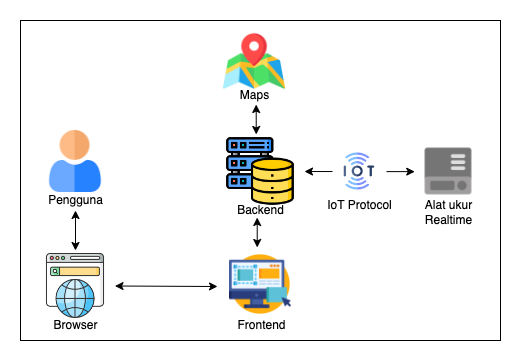
\includegraphics[width=0.8\columnwidth]{bab3/Gambar/web-arsitektur.png}
	\end{center}
	\vspace{-0.2cm}
	%\rule{\columnwidth}{0.1pt}
	\caption{Diagram arsitektur \textit{website} pemantauan kualitas gambar siaran DVB-T2}
	\label{web-arsitektur}
\end{figure}
%%%%%%%%%%%%%%%%%%%%%%%%%% GAMBAR %%%%%%%%%%%%%%%%%%%%%%%%%%%%%%

Laman yang diakses atau diminta, memiliki tampilan antarmuka atau yang dikenal dengan user interface. Front end pada penerapan sistem ini menggunakan \textit{native javascript}. Frontend Native JavaScript merujuk pada pengembangan antarmuka pengguna (user interface) berbasis web yang dibangun menggunakan bahasa pemrograman JavaScript murni tanpa mengandalkan framework atau library tertentu. Frontend Native JavaScript memungkinkan pengembang untuk lebih fleksibel dalam menyesuaikan dan mengubah kode mereka karena mereka memiliki kontrol penuh atas kode tersebut. 

Server yang digunakan pada penelitian ini adalah virtual machine yang terdapat pada server universitas gunadarma. Sistem operasi yang digunakan Ubuntu 22.1 dan \textit{apache} web server. Penyimpanan basis data menggunakan MySQL.  Tampilan Maps yang ditampilkan pada front end merupakan hasil dari permintaan yang terintegrasi terhubung dari Mapbox API. Peta digunakan hanya untuk mengukur jarak antara alat pengukur dengan stasiun pemancar. Kemudian digunakan juga protokol IoT yang berfungsi untuk mengirimkan data pengukuran kualitas sinyal dan gambar ke IoT dashboard yang kemudian API dari IoT tersebut diambil dari web server. Pengguna hanya dapat memilih lokasi pemantauan yang sebelumnya sudah dibuat oleh admin. Lokasi pemantauan merupakan titik dimana perangkat melakukan pengukuran. Selanjutnya data hasil pengukuran ditampilkan secara realtime pada antarmuka web.


